\documentclass[11pt,a4paper]{article}

\usepackage[utf8]{inputenc}
\usepackage[T1]{fontenc}
\usepackage{lmodern}
\usepackage[margin=2.5cm]{geometry}
\usepackage{graphicx}
\usepackage{booktabs}
\usepackage{siunitx}
\usepackage{caption}
\usepackage{subcaption}
\usepackage{hyperref}
\usepackage{amsmath}

\title{Preliminary Model Comparison Results\\[0.5em]
\large NuclearDetonation.jl: Lagrangian Particle Dispersion}
\author{NuclearDetonation.jl}
\date{\today}

\begin{document}
\maketitle

%% ====================================================================
\section{Model Overview}
%% ====================================================================

NuclearDetonation.jl is a Lagrangian particle dispersion model for
simulating atmospheric transport of radioactive debris from nuclear
detonations. Particles are released into a three-dimensional wind field
(ERA5 reanalysis on the full 137-level hybrid sigma-pressure grid) and
advected forward in time, with sub-grid turbulence, gravitational settling,
and dry deposition acting on each particle individually.

Particles are distributed across a three-layer mushroom cloud structure
(lower stem, mid-cap, upper cap) whose geometry and mass fractions are
determined independently for each test by BIPOP-CMA-ES optimisation against
digitised fallout observations. The test-specific release geometries are
shown in Sections~\ref{sec:nancy} and~\ref{sec:smoky}.

\subsection{Ornstein--Uhlenbeck Turbulence}

Atmospheric turbulence is represented by an Ornstein--Uhlenbeck (OU)
stochastic process \cite{uhlenbeck1930} rather than a simple random walk. In a random walk, each
turbulent velocity perturbation is drawn independently at every timestep,
producing unrealistically jagged trajectories. The OU process treats the
turbulent velocity as a variable with temporal memory: it decays
exponentially towards zero with a Lagrangian timescale $\tau_L$, while a
stochastic forcing term continually injects energy:
\begin{equation}
    u'(t + \Delta t) = u'(t)\,\exp\!\bigl(-\Delta t / \tau_L\bigr)
    + \sigma_u \sqrt{1 - \exp\!\bigl(-2\,\Delta t / \tau_L\bigr)}\;\xi,
\end{equation}
where $\sigma_u$ is the turbulent velocity standard deviation and
$\xi \sim \mathcal{N}(0,1)$. The standard deviations $\sigma_u$,
$\sigma_v$, $\sigma_w$ and timescales $\tau_L$ are computed from the Hanna
(1982) parameterisation, which uses boundary-layer stability class and
height above ground. Separate OU processes are maintained for the horizontal
and vertical components.

The practical effect is that particles ``remember'' their turbulent velocity
over timescales of tens of seconds to minutes, producing smoother, more
physically plausible dispersion than an uncorrelated walk.

\subsection{Gravitational Settling}

Each particle is assigned a diameter drawn from a bimodal lognormal
distribution (fine and coarse fractions), representing the range of debris
sizes from sub-micron fission products to hundreds-of-micron soil
particles. The gravitational settling velocity for each particle is computed
from Stokes drag with a Cunningham slip correction \cite{cunningham1910} for small particles:
\begin{equation}
    v_g = \frac{\rho_p\, d_p^2\, g\, C_s}{18\,\mu}
\end{equation}
where $\rho_p$ is the particle density, $d_p$ is the diameter, $\mu$ is the
dynamic viscosity of air (Sutherland's formula \cite{sutherland1893}, temperature-dependent), and
$C_s$ is the Cunningham slip correction factor:
\begin{equation}
    C_s = 1 + \frac{2\lambda}{d_p}\left(1.257 + 0.4\,\exp\!\left(-\frac{0.55\,d_p}{\lambda}\right)\right)
\end{equation}
with $\lambda$ the mean free path of air. The settling velocity is added to
the vertical component of the particle velocity at each timestep, so large
particles fall out quickly and deposit close to ground zero whilst fine
particles remain aloft and travel long distances.

\subsection{Dry Deposition}

Surface removal of particles uses a resistance analogy following Zhang et
al.~\cite{zhang2001}. The deposition velocity is:
\begin{equation}
    v_d = v_g + \frac{1}{R_a + R_s}
\end{equation}
where $R_a$ is the aerodynamic resistance (from Monin--Obukhov similarity
theory, accounting for atmospheric stability) and $R_s$ is the surface
resistance. The surface resistance depends on three collection mechanisms:
Brownian diffusion ($E_B \propto \mathrm{Sc}^{-0.54}$), inertial impaction
($E_{\mathrm{IM}}$ via the Stokes number), and interception ($E_{\mathrm{IN}}$
via the ratio of particle diameter to collector radius). A rebound correction
$R_1 = 1 - \exp(-\sqrt{\mathrm{St}})$ accounts for particles bouncing off
surfaces rather than sticking.

When a particle's height drops below a threshold near the surface, its mass
is reduced exponentially at a rate $k = v_d / h_{\mathrm{mix}}$, transferring
activity to the ground-level deposition field.

\clearpage
%% ====================================================================
\section{Nancy 24\,kT: Consortium Comparison}
\label{sec:nancy}
%% ====================================================================

Figure~\ref{fig:nancy_cloud} shows the three-layer release geometry for the
Nancy test, derived from NOAA~1984 debris cloud observations. The BIPOP-CMA-ES
optimisation places 5.6\% of activity in the lower stem (0--3.8\,km),
35.1\% in the mid-cap (3.8--6.1\,km), and 59.3\% in the upper cap
(6.1--12.5\,km). The Glasstone \& Dolan (1977) empirical cloud dimensions
for 24\,kT provide the wireframe outline.

\begin{figure}[htbp]
\centering
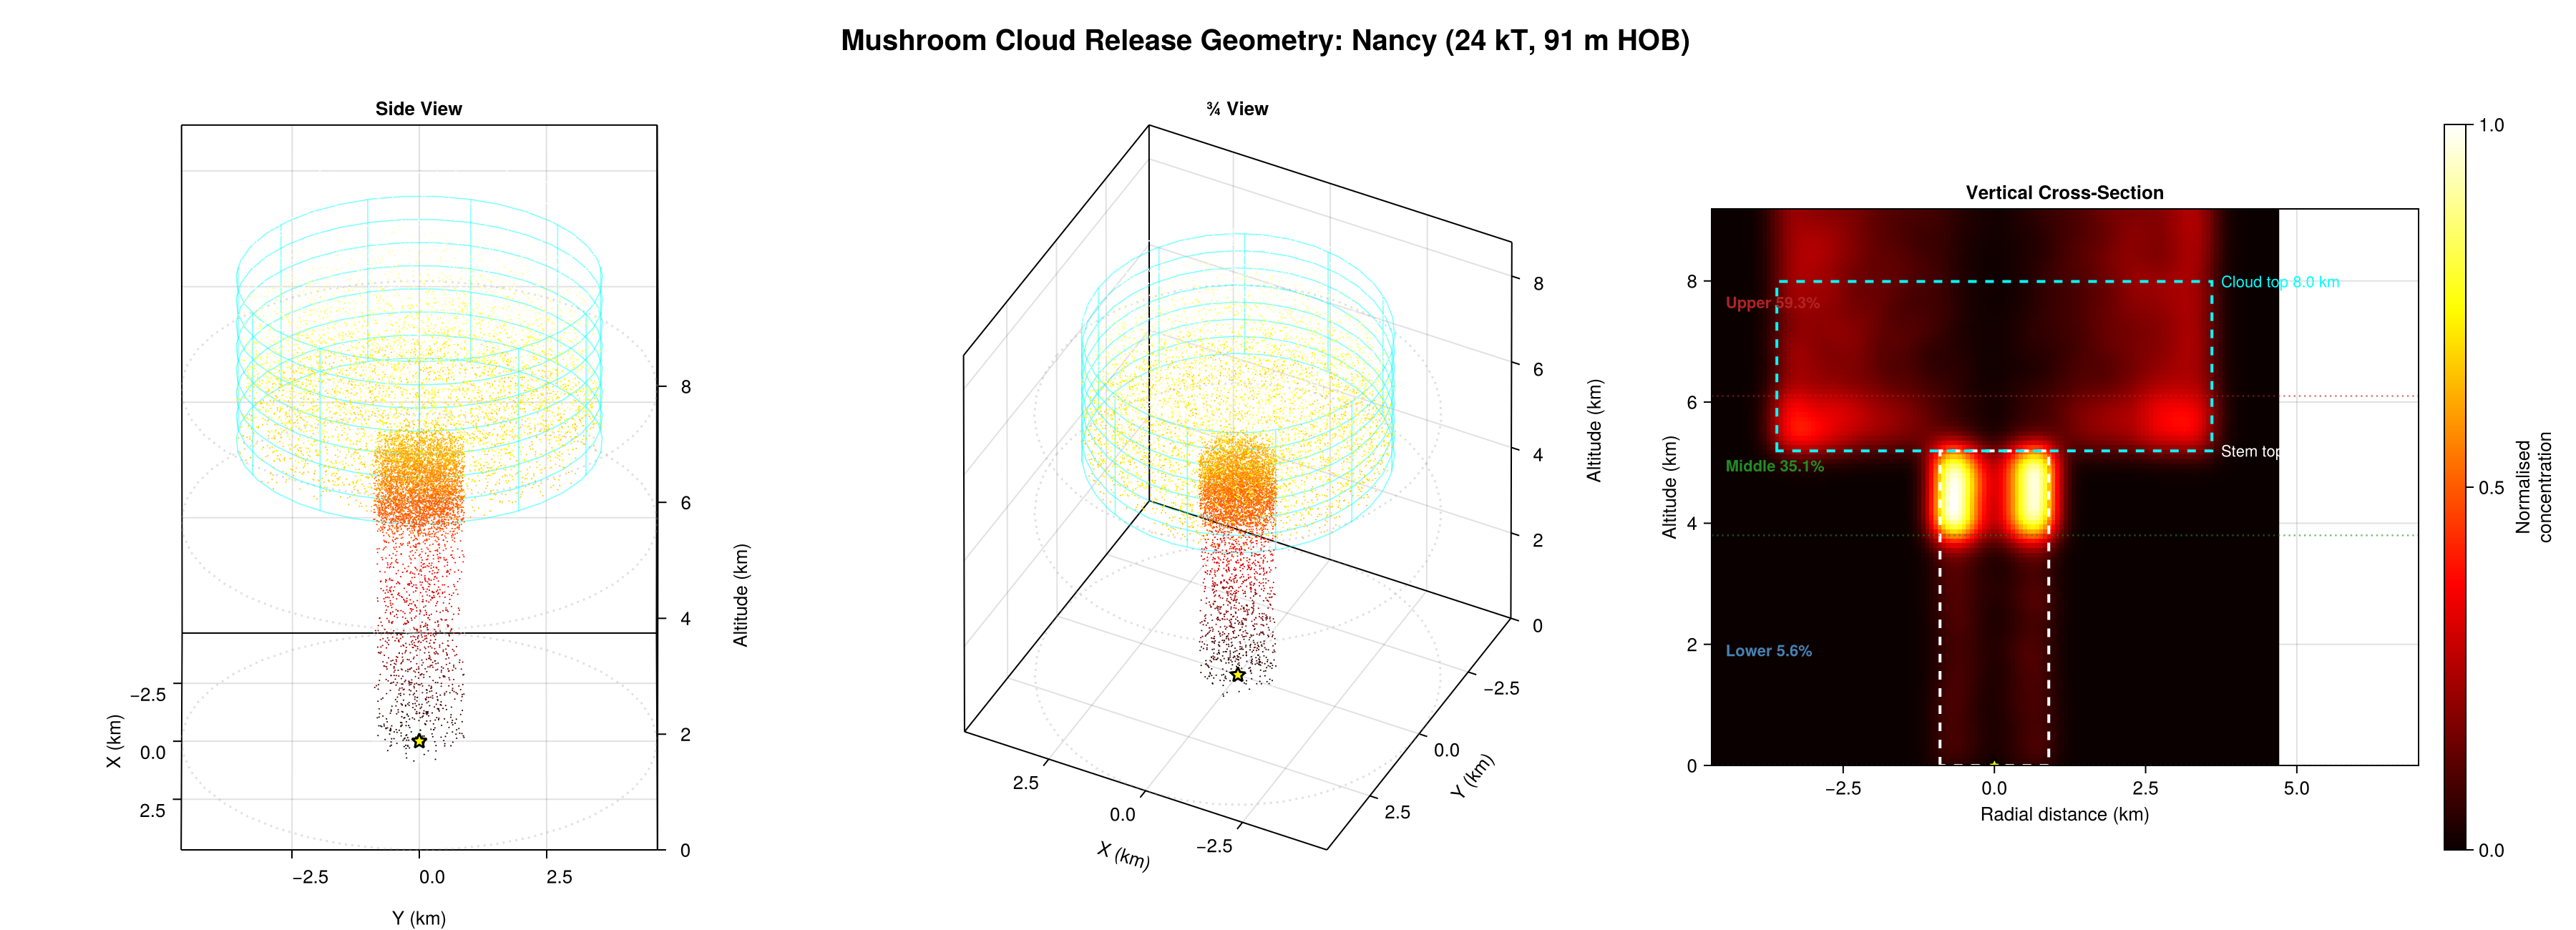
\includegraphics[width=\textwidth]{nancy_mushroom_cloud.png}
\caption{Nancy 24\,kT release geometry. Three-layer particle distribution
(lower 5.6\%, middle 35.1\%, upper 59.3\%) with Glasstone \& Dolan
wireframe. Left/centre: 3D views; right: vertical cross-section with
kernel density concentration field.}
\label{fig:nancy_cloud}
\end{figure}

The model was first validated against the Upshot-Knothole Nancy test
(24\,kT, 24 March 1953). Simulated dose rate contours at H+12 hours are
compared with digitised observations using the Figure of Merit in Space:
\begin{equation}
    \mathrm{FMS} = \frac{A_{\text{obs}} \cap A_{\text{model}}}{A_{\text{obs}} \cup A_{\text{model}}}
\end{equation}
Six dose rate thresholds are evaluated: 0.4, 1, 4, 10, 40, and
100\,mR/h. Each consortium member submitted output in their native format,
interpolated onto a common 2\,km grid for scoring.

Table~\ref{tab:nancy_fms} summarises the results. Our model achieves a mean
FMS of 45.9\%, roughly 17 percentage points above the next-best consortium
member (UKMO, 28.8\%).

\begin{table}[htbp]
\centering
\caption{FMS scores for Nancy 24\,kT at H+12.}
\label{tab:nancy_fms}
\begin{tabular}{lrrrrrr}
\toprule
Dose Rate (mR/h) & Our Model & UKMO & BfS & KIT & DSA/MET & DEMA \\
\midrule
0.4 & 67.1\% & 60.4\% & 52.9\% & 33.8\% & 45.6\% & 0.7\% \\
1 & 58.7\% & 47.3\% & 31.1\% & 27.7\% & 28.1\% & -- \\
4 & 55.6\% & 22.4\% & 18.2\% & 18.9\% & 16.9\% & -- \\
10 & 40.1\% & 15.9\% & 9.9\% & 12.1\% & 9.2\% & -- \\
40 & 28.7\% & 16.2\% & 5.4\% & 4.4\% & 5.5\% & -- \\
100 & 25.2\% & 10.5\% & 2.8\% & 0.5\% & 2.2\% & -- \\
\midrule
Mean & \textbf{45.9\%} & \textbf{28.8\%} & \textbf{20.0\%} & \textbf{16.2\%} & \textbf{17.9\%} & \textbf{0.1\%} \\
\bottomrule
\end{tabular}
\end{table}

\clearpage
%% ====================================================================
\section{Side-by-Side Comparisons}
%% ====================================================================

The following figures show the digitised observation contours (left panel) and
each model's predicted dose rate contours (right panel) for the six
thresholds.

\begin{figure}[htbp]
\centering
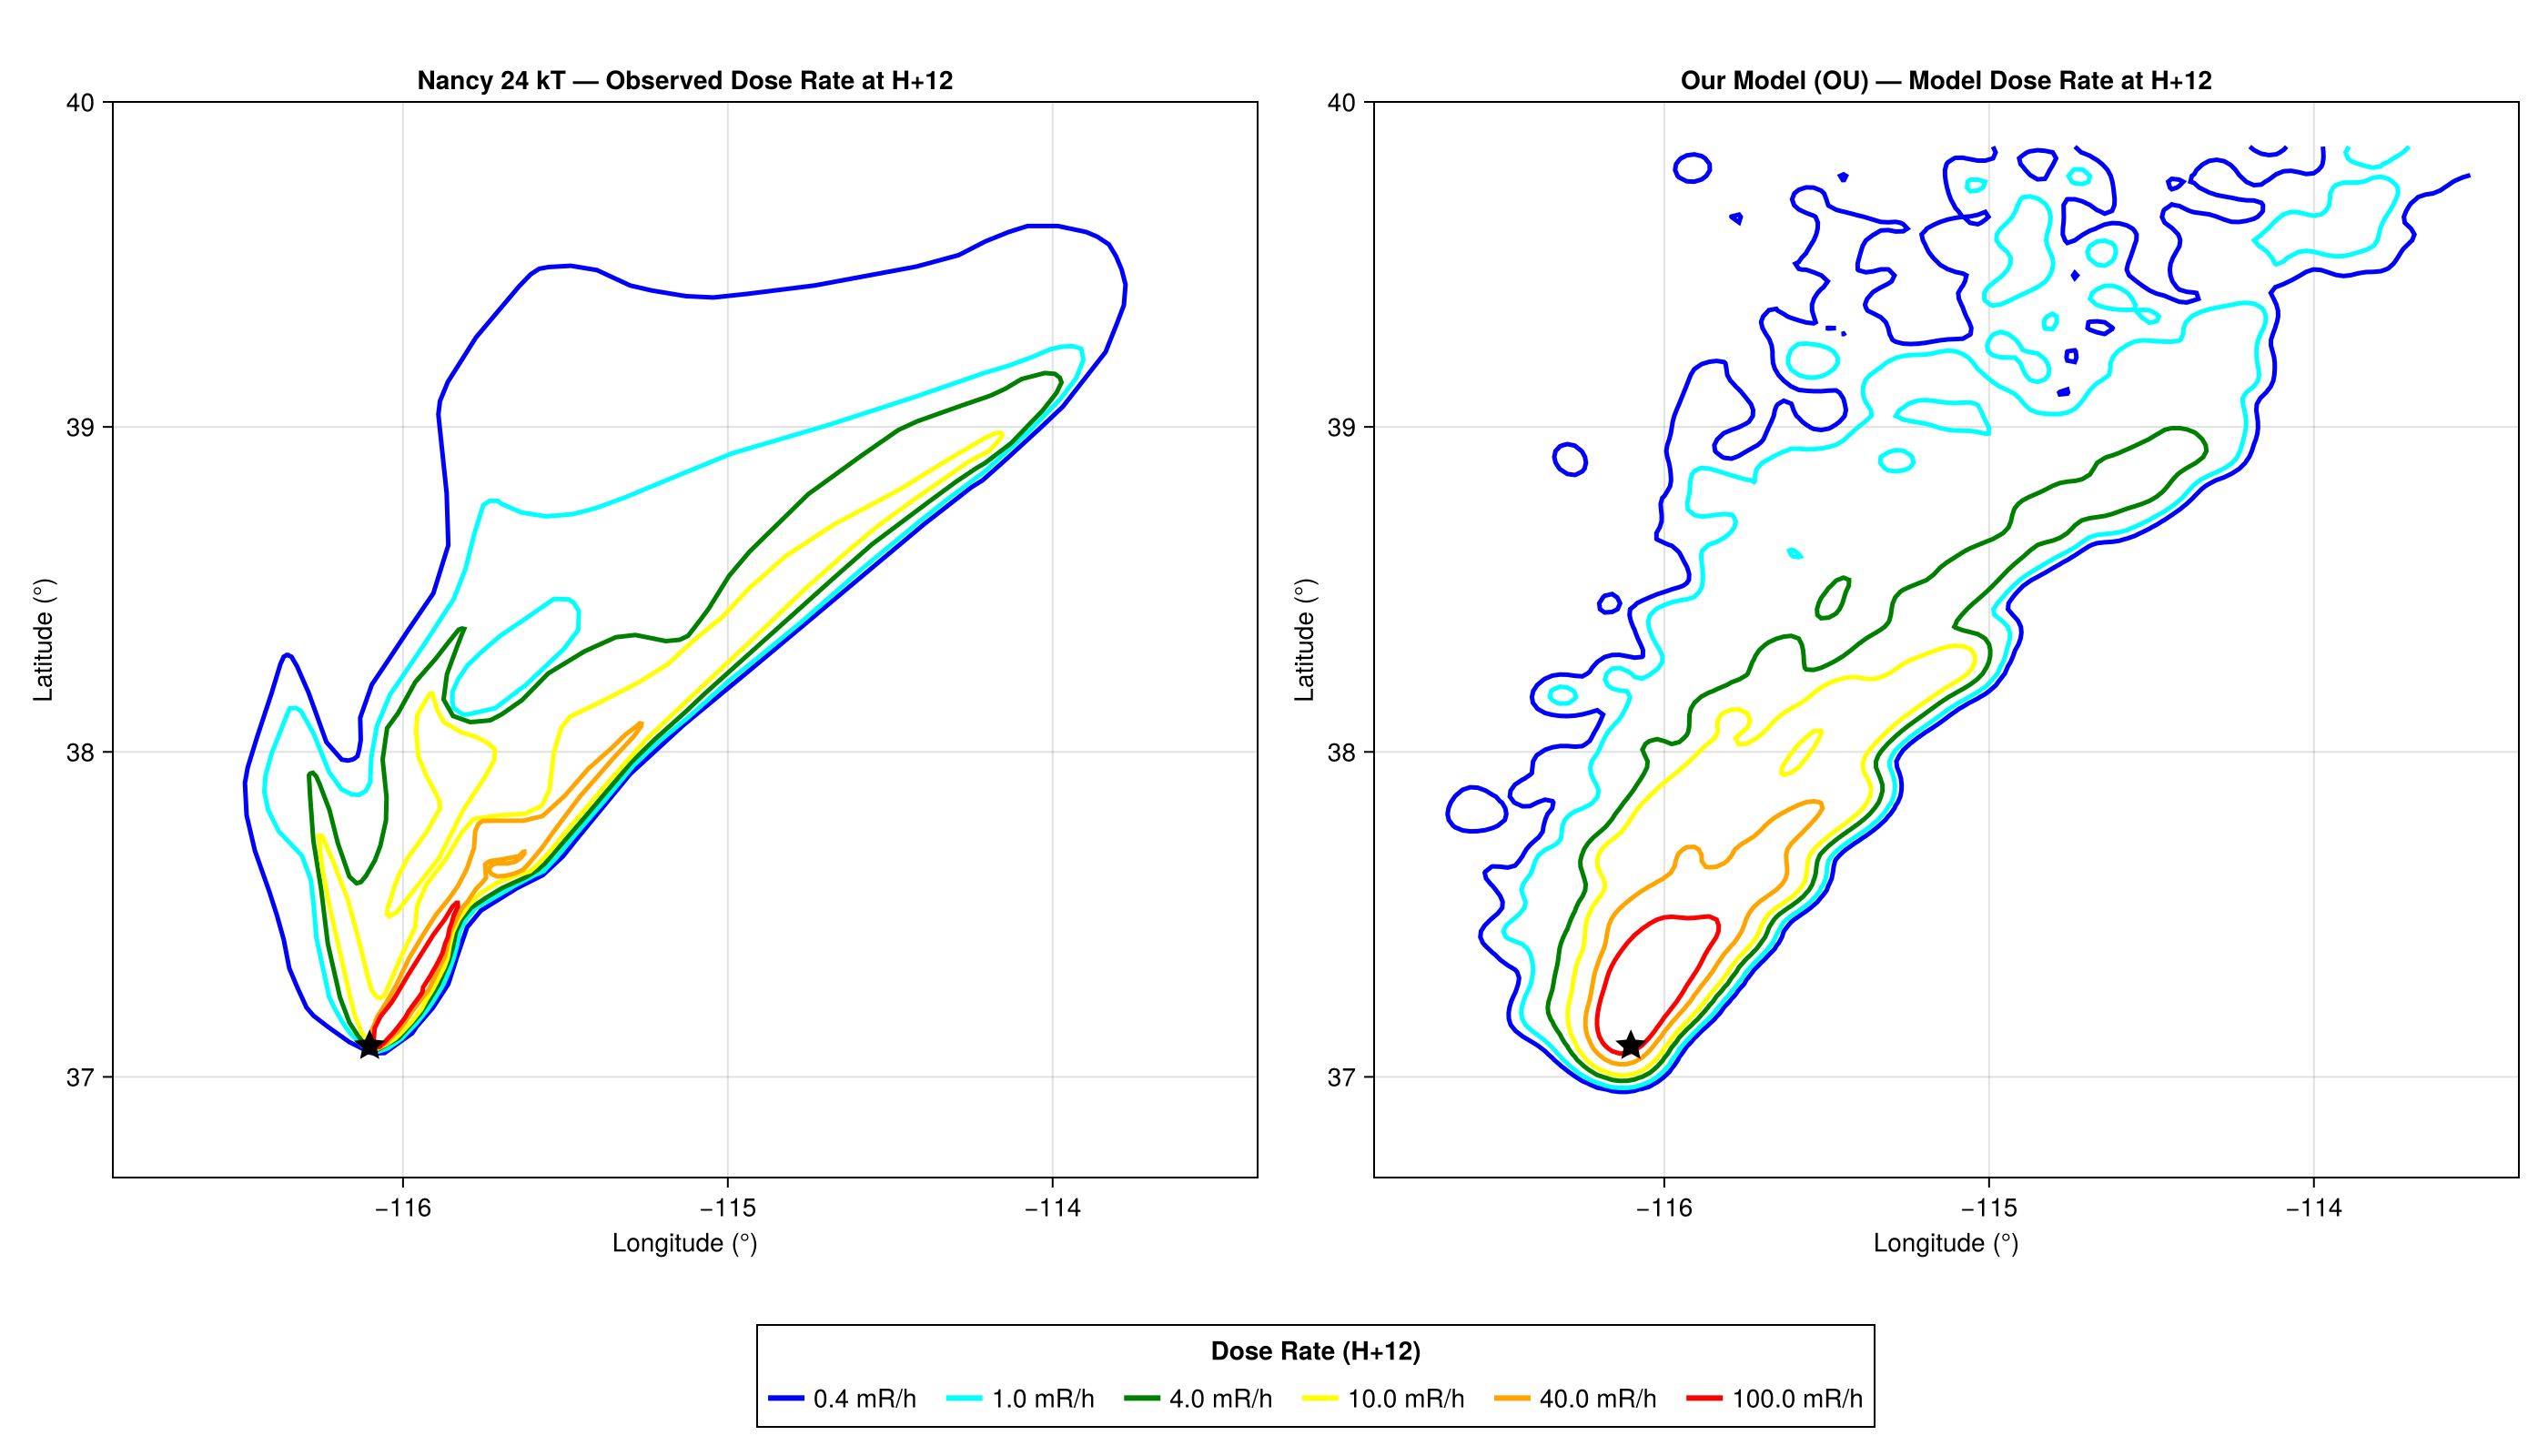
\includegraphics[width=\textwidth]{nancy_fms_OurModel.png}
\caption{Nancy FMS comparison: our model (right) vs digitised observations
(left) for six dose rate thresholds. Mean FMS 45.9\%.}
\label{fig:fms_ours}
\end{figure}

\begin{figure}[htbp]
\centering
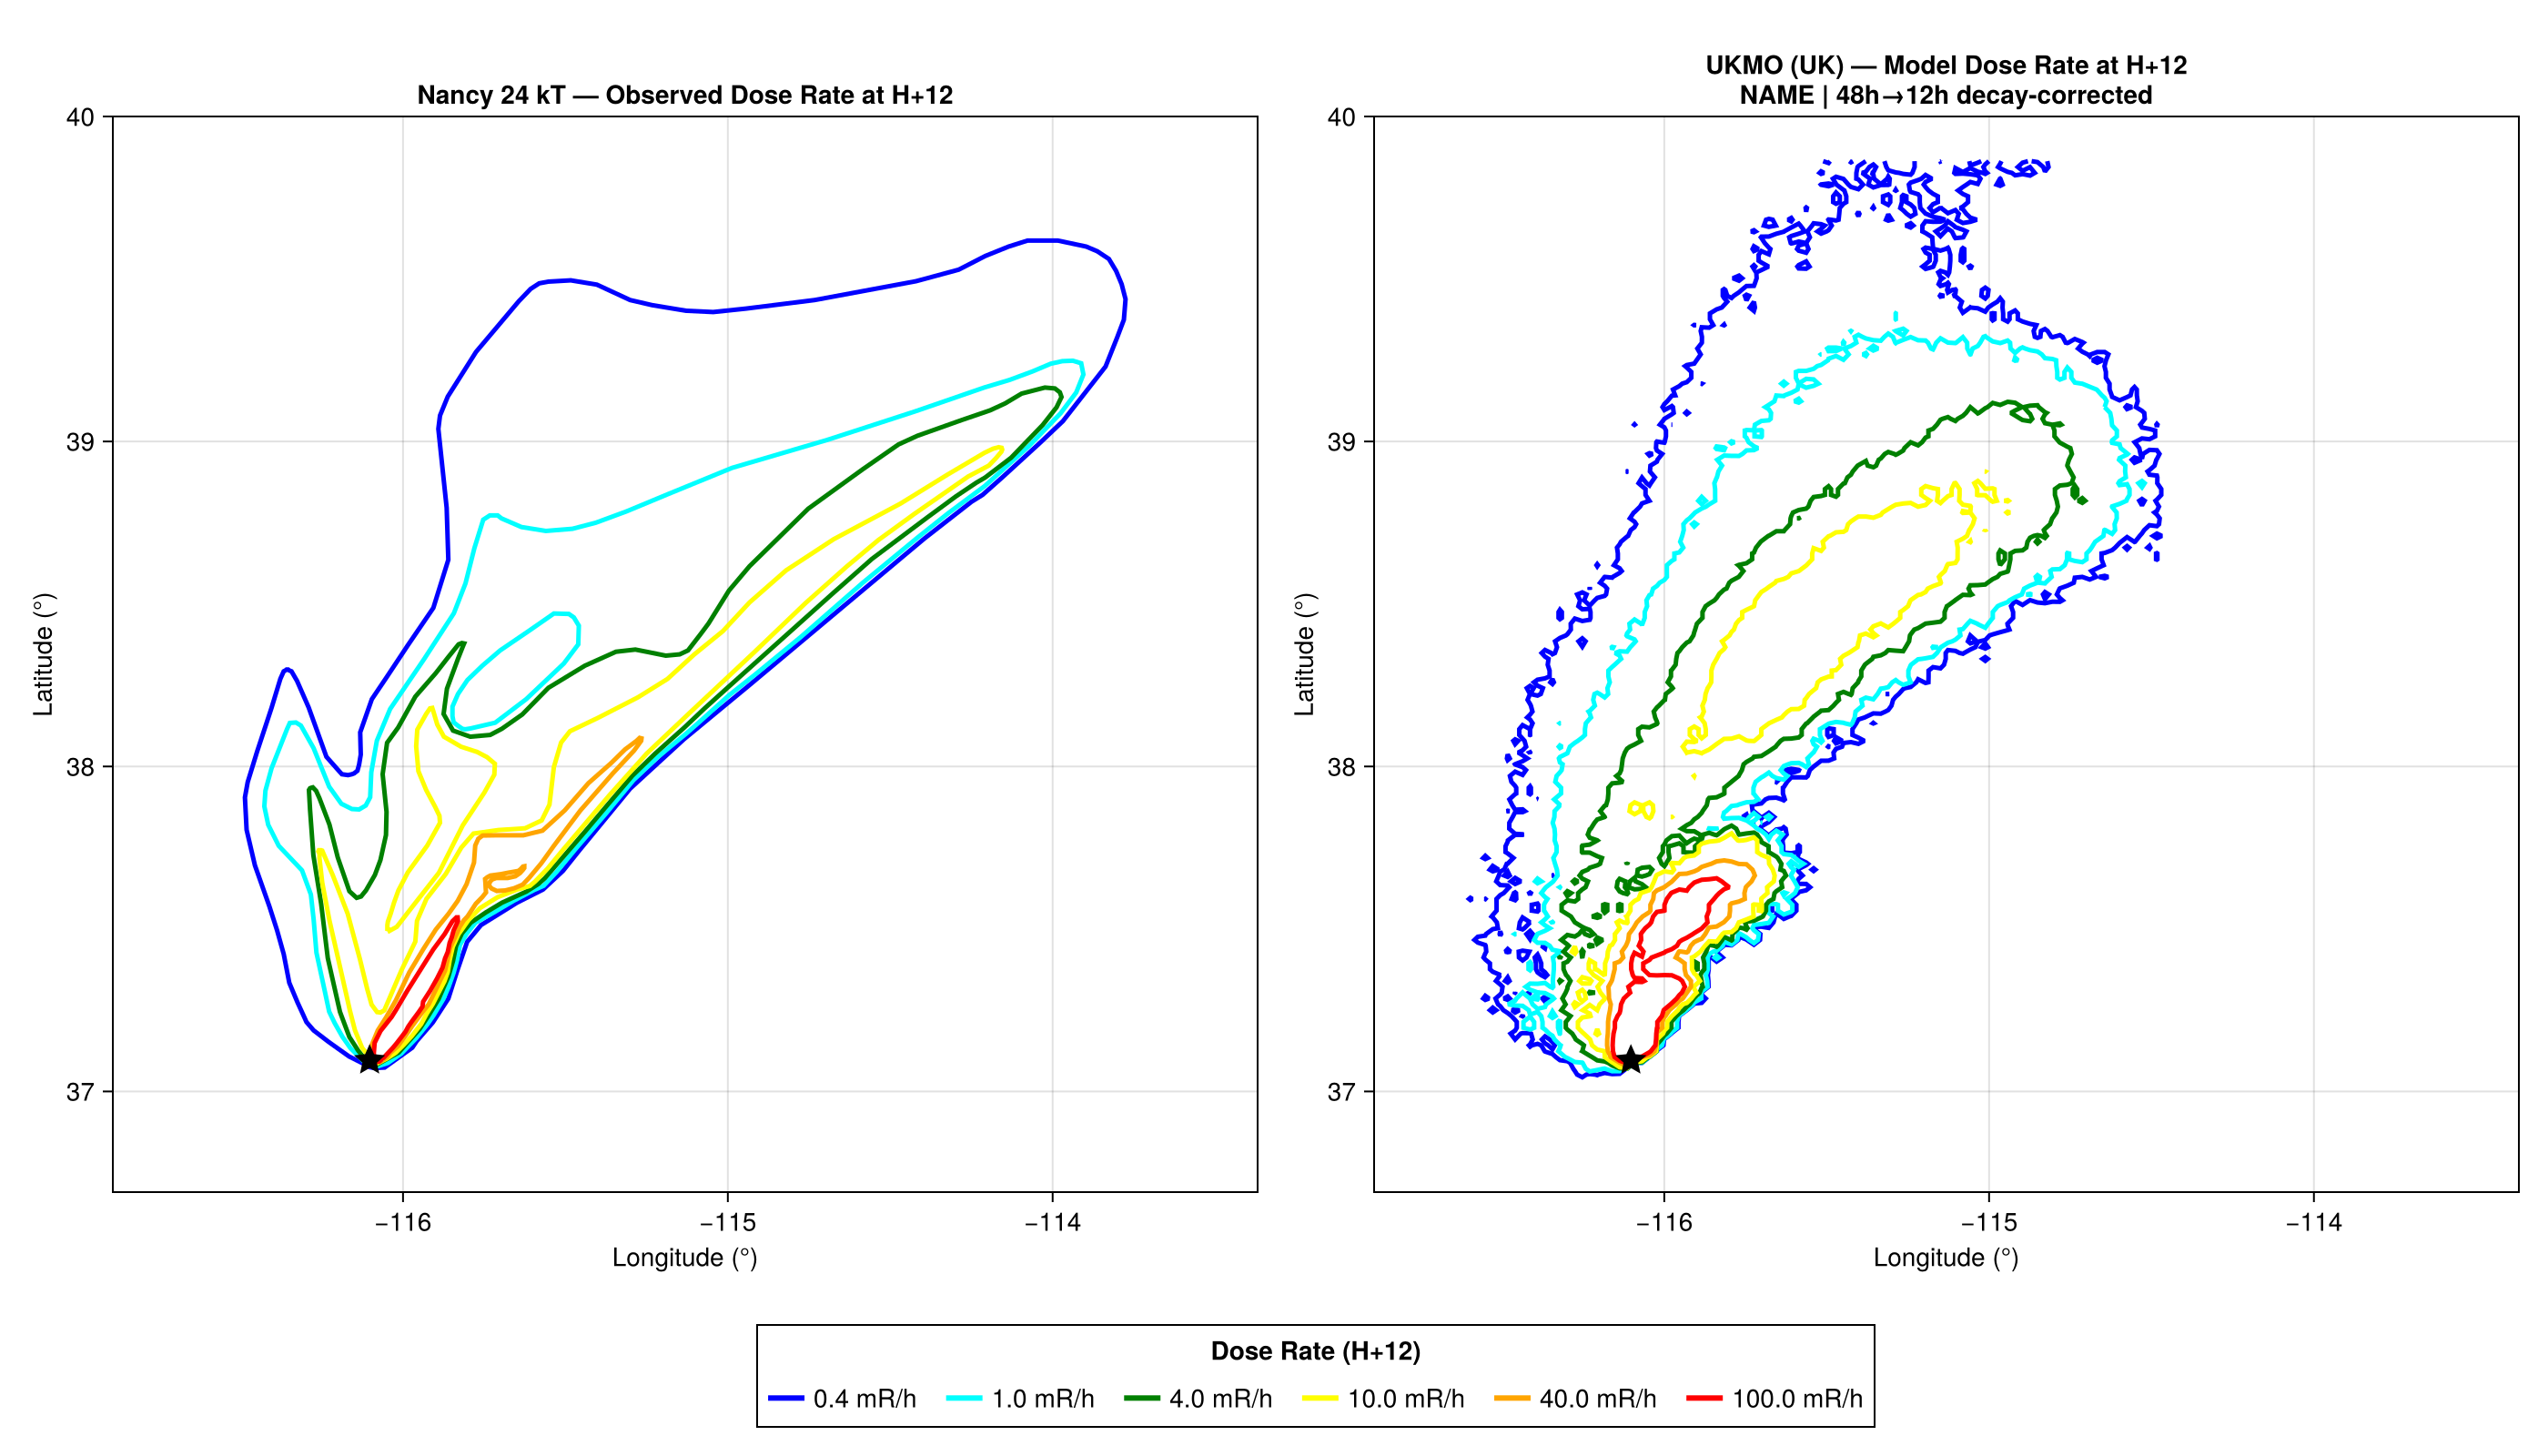
\includegraphics[width=\textwidth]{nancy_fms_UKMO.png}
\caption{Nancy FMS comparison: UKMO, UK Met Office NAME model (right) vs
digitised observations (left). Mean FMS 28.8\%.}
\label{fig:fms_ukmo}
\end{figure}

\begin{figure}[htbp]
\centering
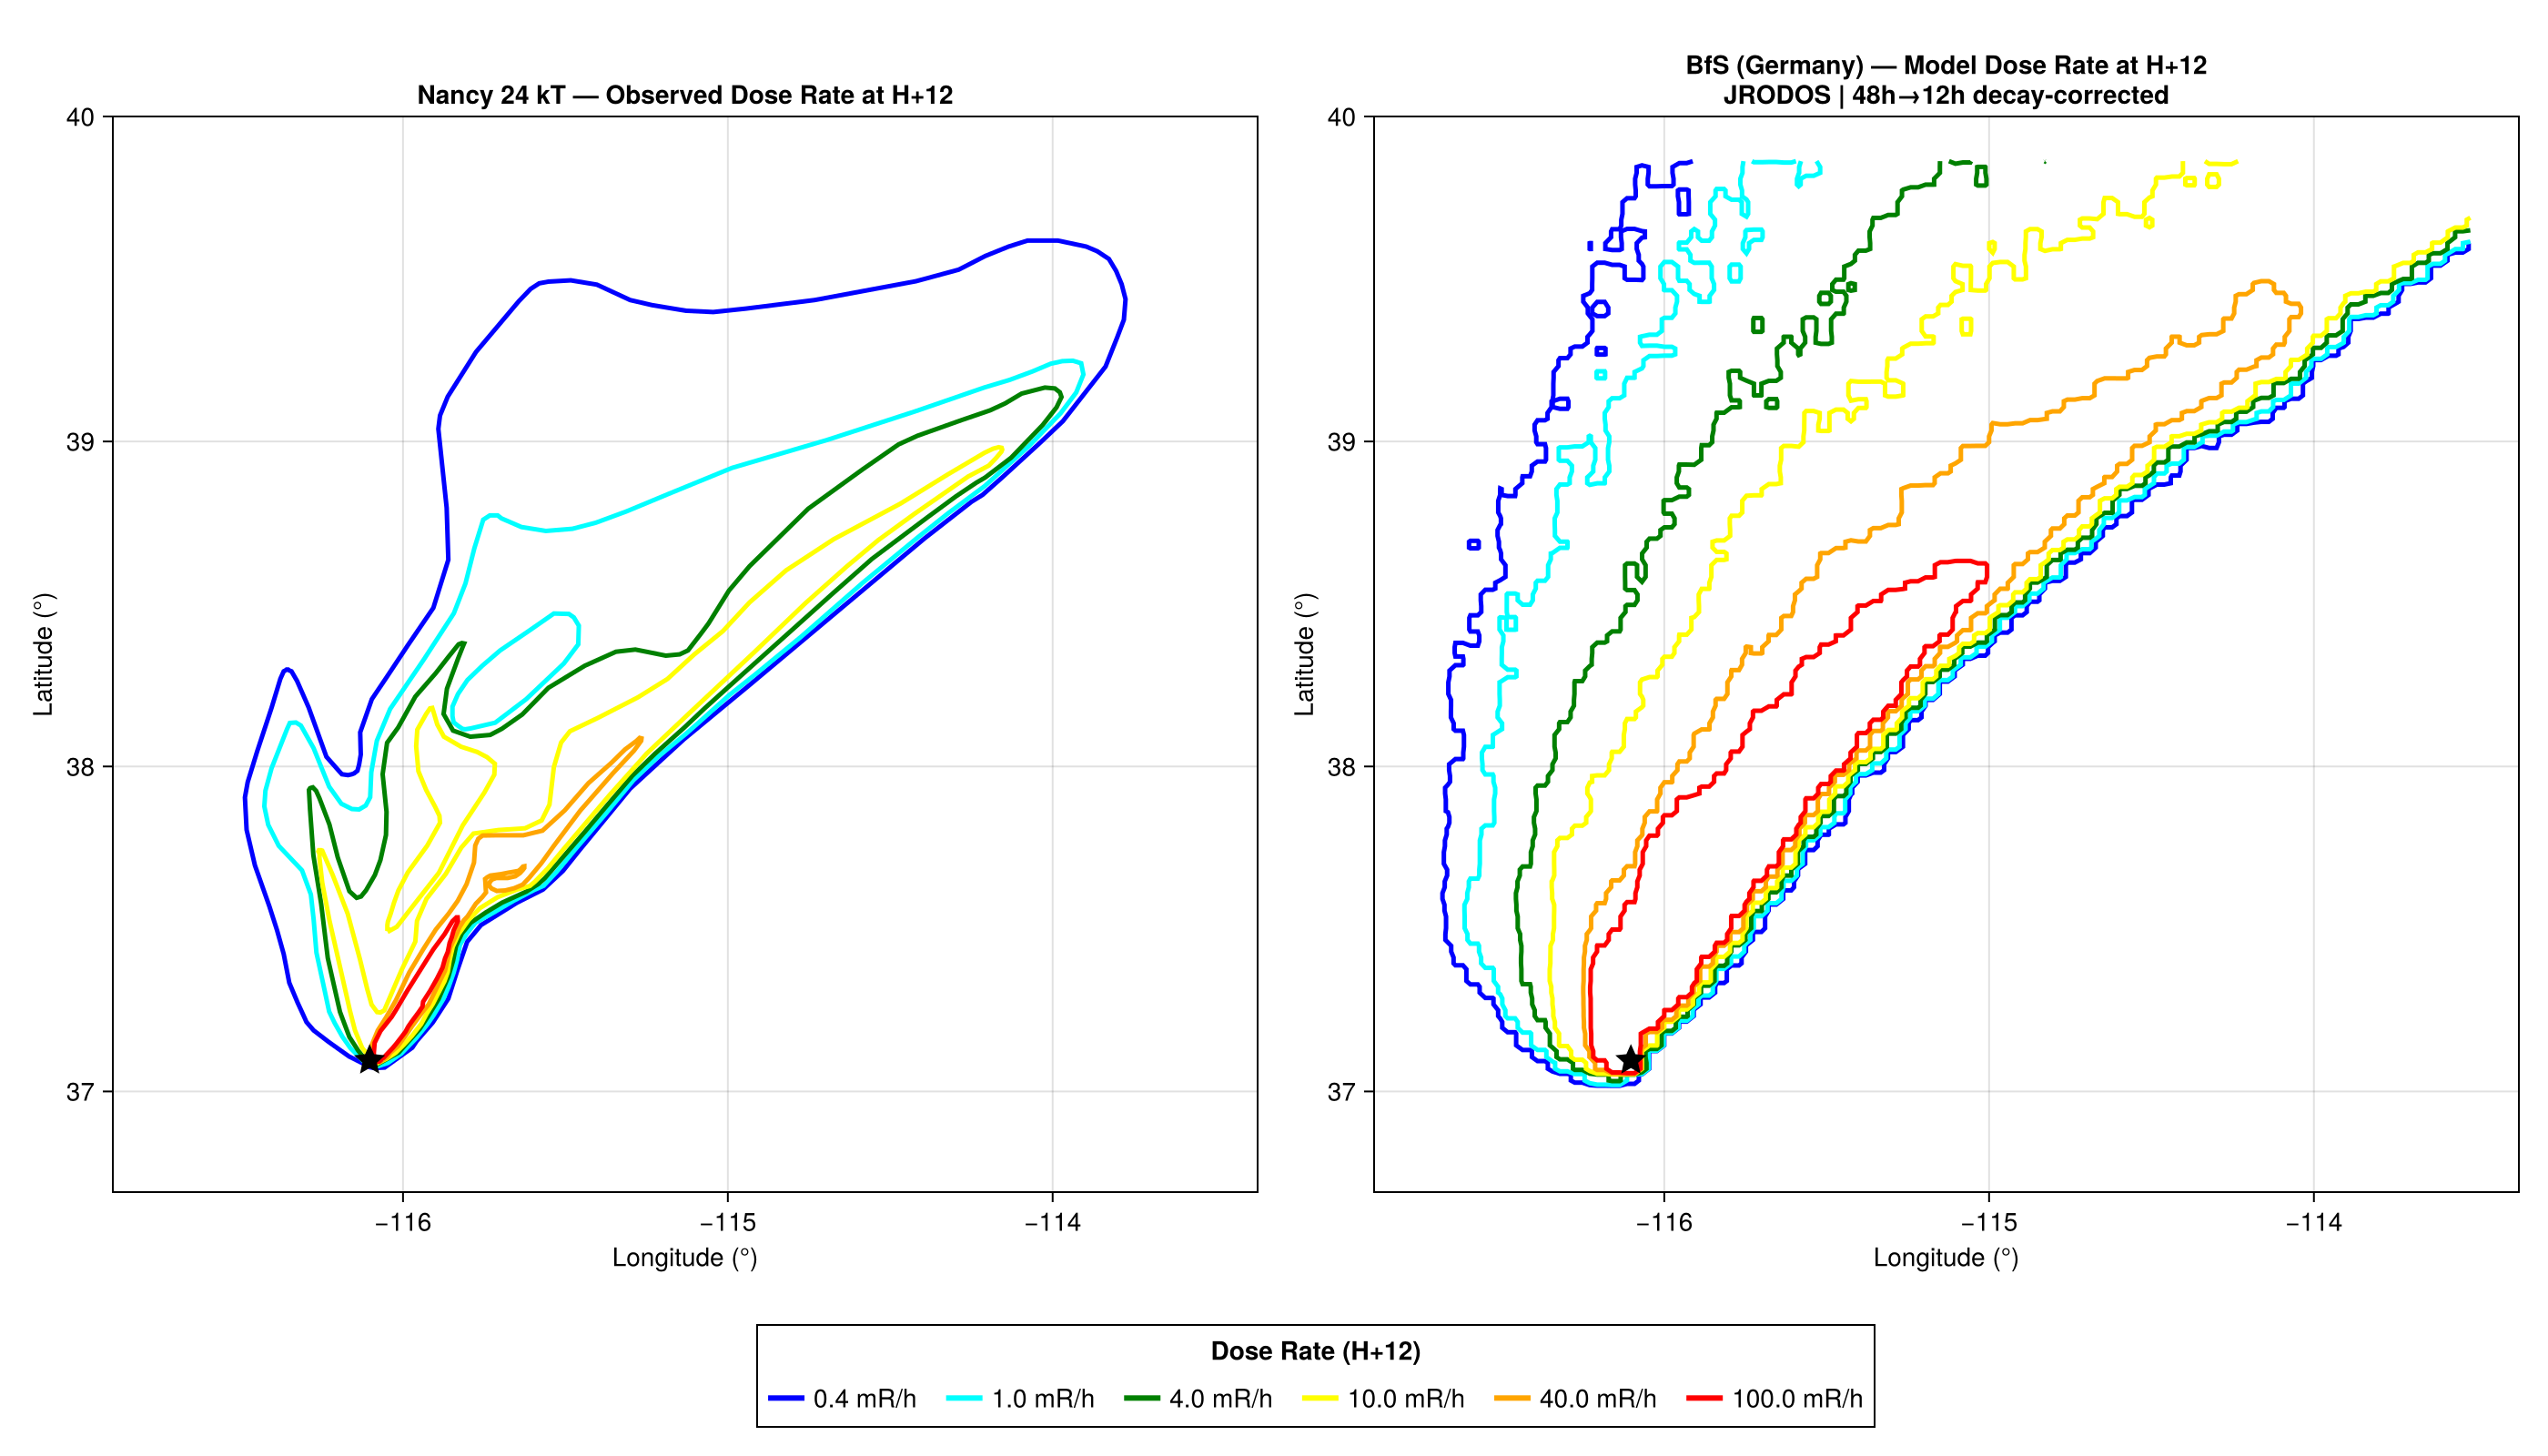
\includegraphics[width=\textwidth]{nancy_fms_BfS.png}
\caption{Nancy FMS comparison: BfS, Germany, JRODOS (right) vs digitised
observations (left). Mean FMS 20.0\%.}
\label{fig:fms_bfs}
\end{figure}

\begin{figure}[htbp]
\centering
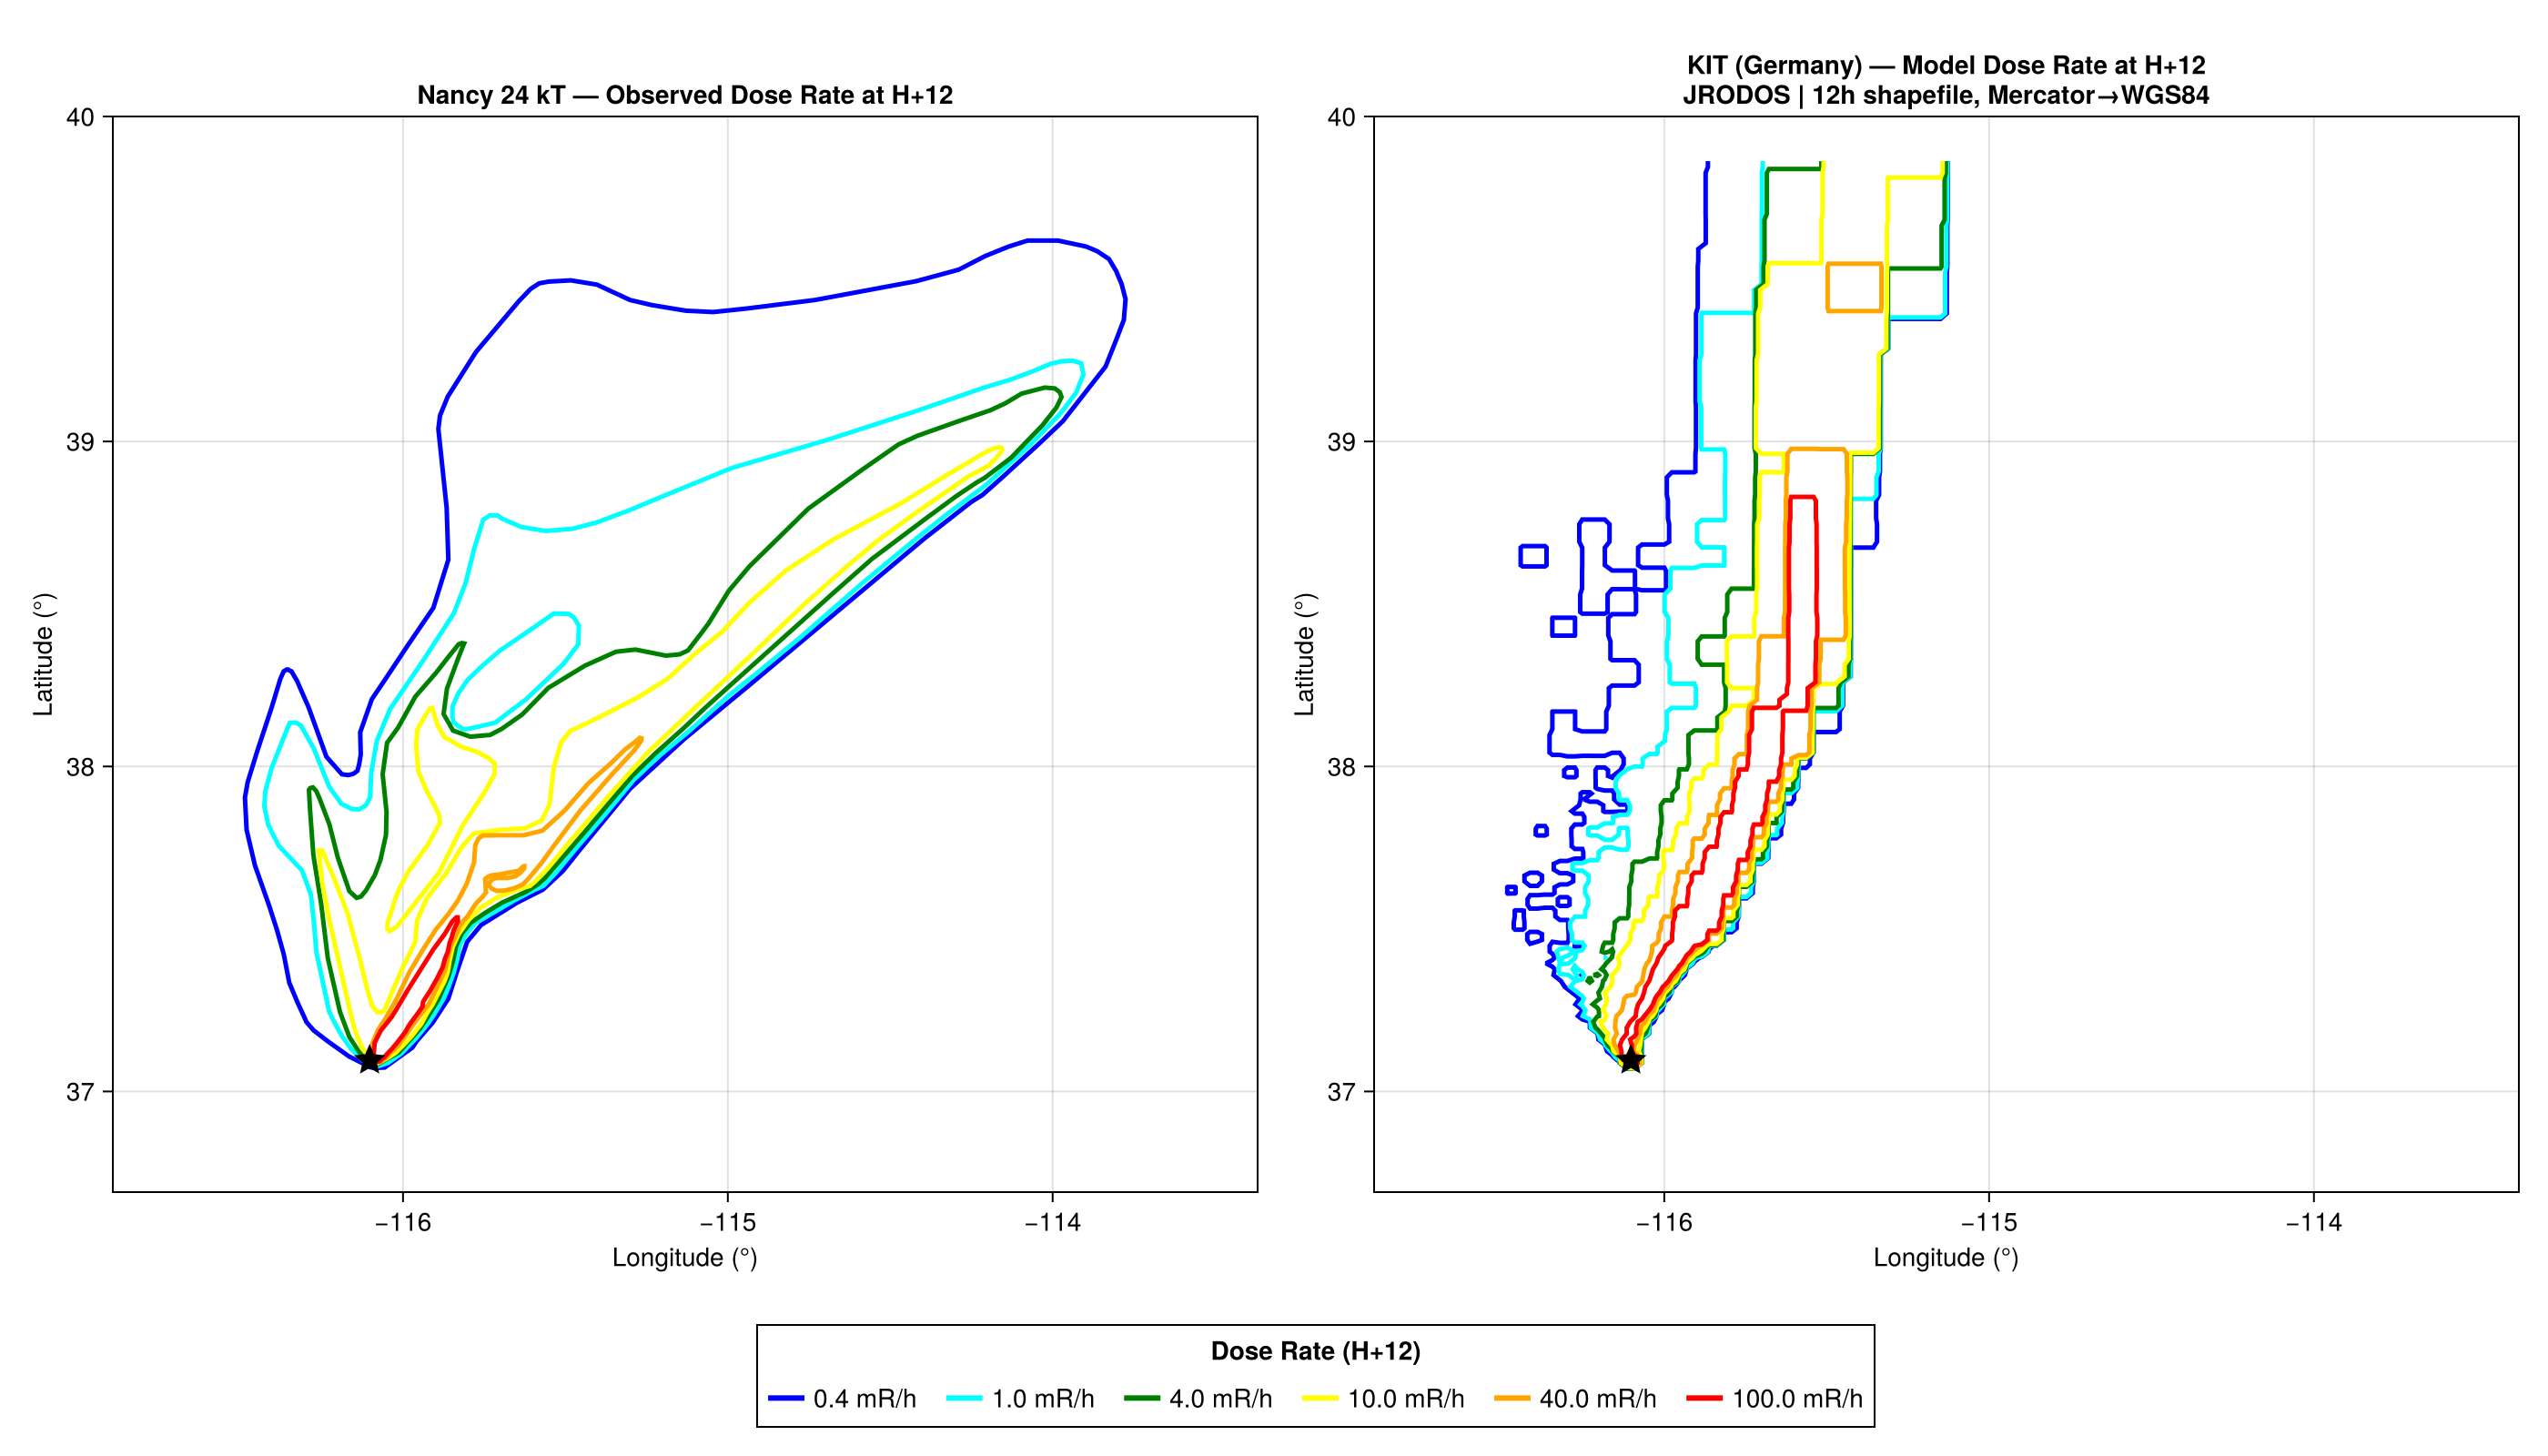
\includegraphics[width=\textwidth]{nancy_fms_KIT.png}
\caption{Nancy FMS comparison: KIT, Germany, JRODOS (right) vs digitised
observations (left). Mean FMS 16.2\%.}
\label{fig:fms_kit}
\end{figure}

\begin{figure}[htbp]
\centering
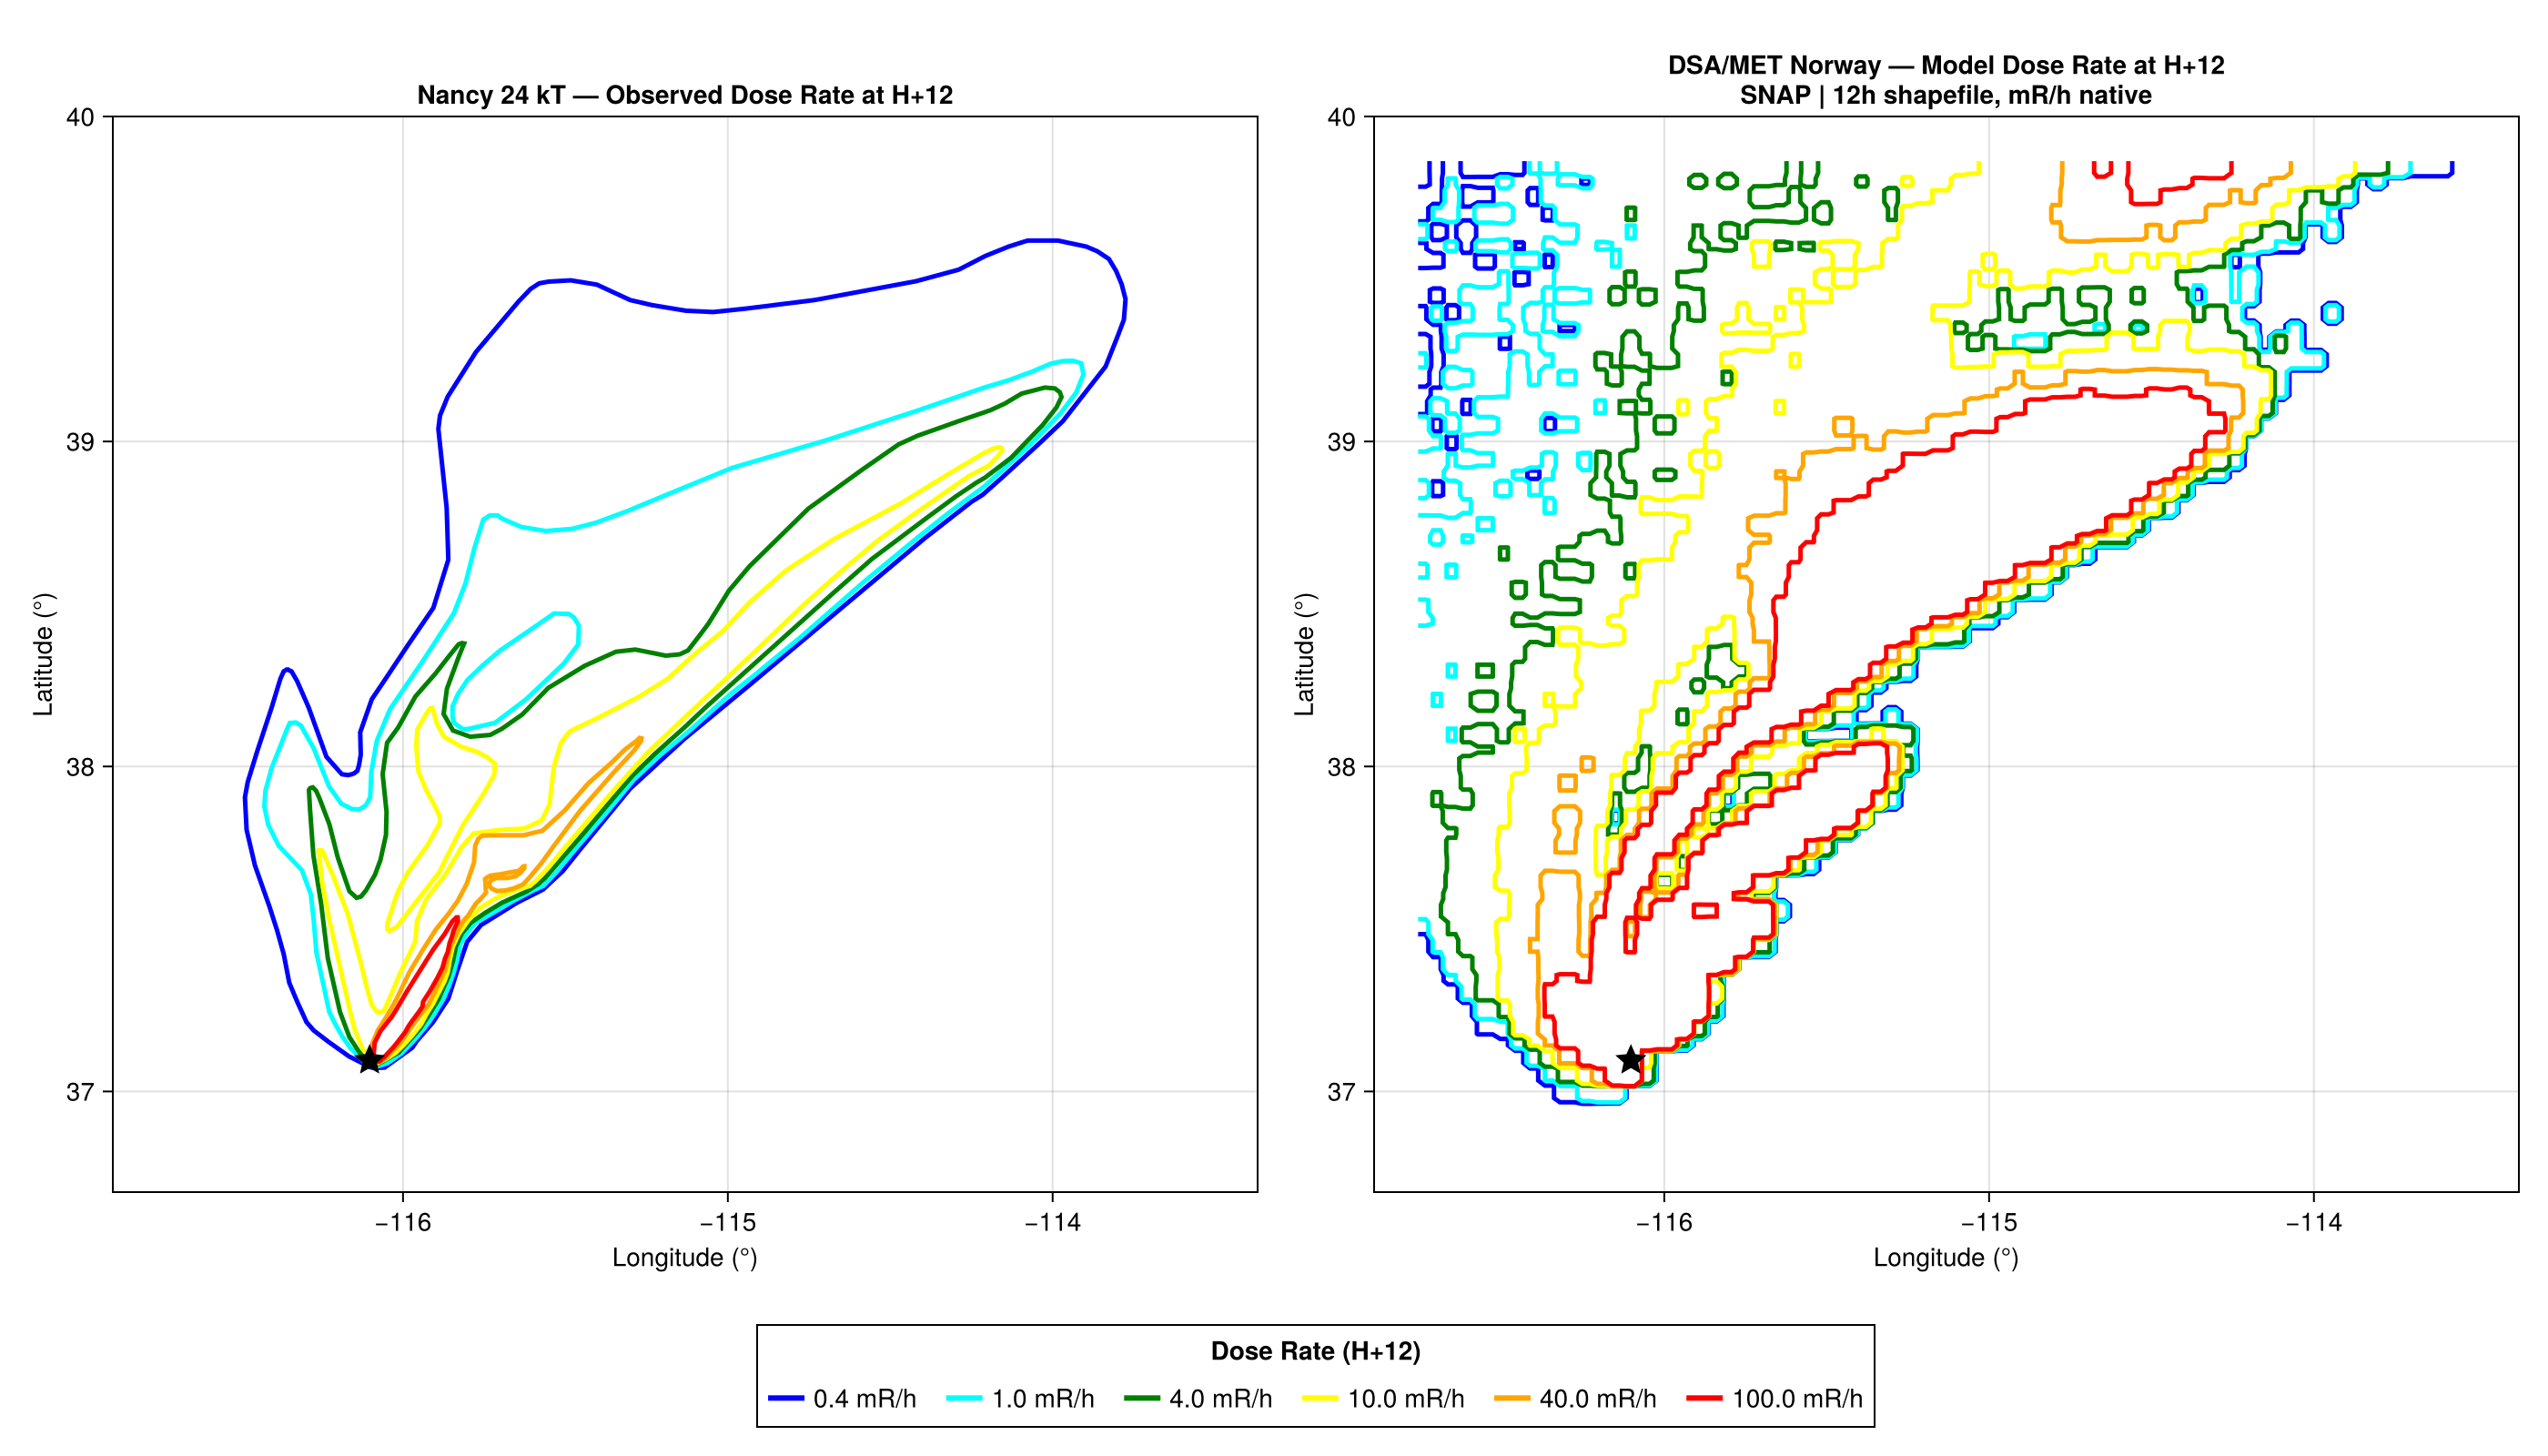
\includegraphics[width=\textwidth]{nancy_fms_DSA.png}
\caption{Nancy FMS comparison: DSA/MET Norway, SNAP model (right) vs
digitised observations (left). Mean FMS 17.9\%.}
\label{fig:fms_dsa}
\end{figure}

\begin{figure}[htbp]
\centering
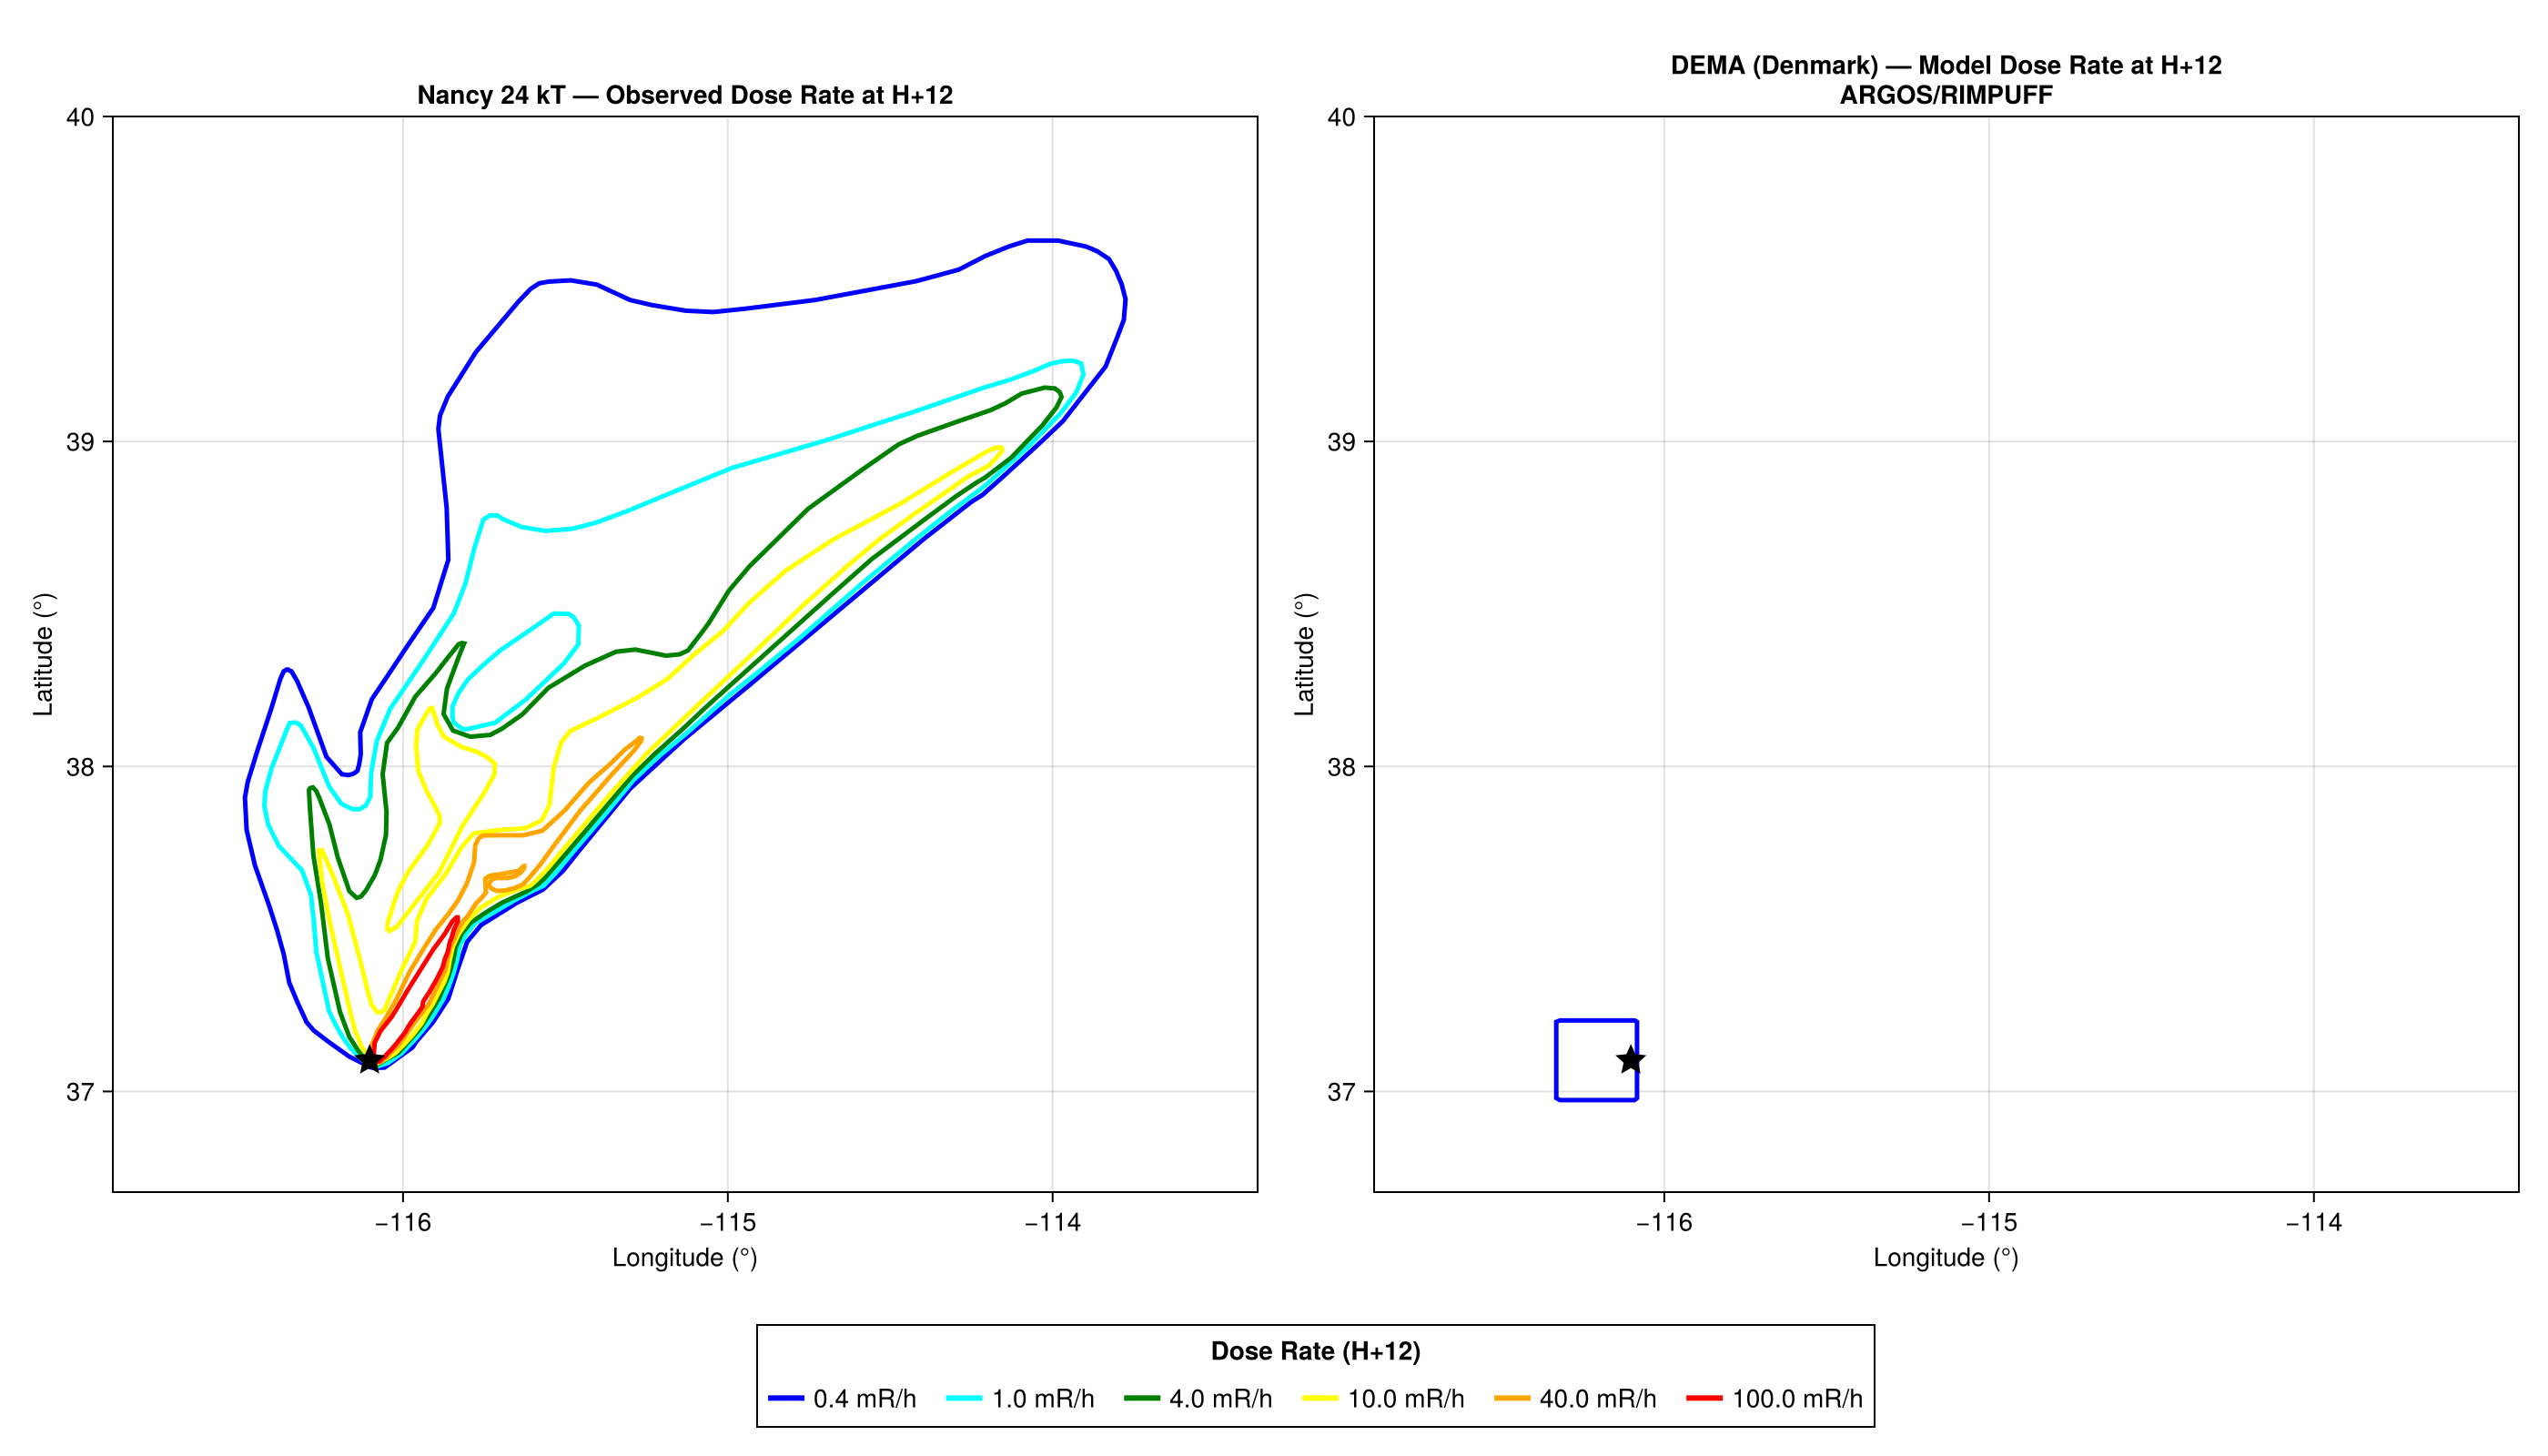
\includegraphics[width=\textwidth]{nancy_fms_DEMA.png}
\caption{Nancy FMS comparison: DEMA, Denmark, ARGOS/RIMPUFF (right) vs
digitised observations (left). Mean FMS 0.1\%.}
\label{fig:fms_dema}
\end{figure}

\clearpage
%% ====================================================================
\section{Nancy 24\,kT: Observed vs Model}
%% ====================================================================

Figure~\ref{fig:nancy_obs_model} shows a direct comparison between
digitised observations and model predictions for the Nancy test. The top row
compares dose rate contours at H+12; the bottom row compares time-of-arrival
(TOA) contours showing when the fallout plume first reached each location.
The model TOA is computed from cumulative hourly deposition snapshots,
smoothed with a Gaussian kernel and thresholded at 0.1\% of the peak to
detect the advancing plume front.

\begin{figure}[htbp]
\centering

\includegraphics[width=\textwidth]{nancy_bomb_release.png}
\caption{Nancy 24\,kT: observed (left) vs model (right). Top row: dose
rate contours at H+12 for six thresholds (0.4, 1, 4, 10, 40,
100\,mR/h). Bottom row: time-of-arrival contours showing plume
progression from H+1 through H+7.}
\label{fig:nancy_obs_model}
\end{figure}

\clearpage
%% ====================================================================
\section{Smoky 44\,kT: Preliminary Results}
\label{sec:smoky}
%% ====================================================================

The same model and OU turbulence scheme were applied to the Plumbbob Smoky
test (44\,kT tower shot, 31 August 1957, Nevada Test Site). Unlike Nancy,
where the three-layer boundaries are fixed from NOAA~1984 observations,
Smoky's layer heights were included as tuneable parameters in the CMA-ES
optimisation. The best-fit cloud geometry (Figure~\ref{fig:smoky_cloud})
places the stem top at 1.7\,km, cap midpoint at 7.4\,km, and cloud top at
10.4\,km AGL, with 16.9\% of activity in the lower stem, 6.5\% in the
mid-cap, and 76.6\% in the upper cap. The thin grey wireframe in
Figure~\ref{fig:smoky_cloud} shows the Glasstone \& Dolan empirical cloud
for comparison; the optimiser infers a broader mid-cap region and a higher
cloud top than the empirical formulae predict. ERA5 reanalysis provides
the driving meteorology.

\begin{figure}[htbp]
\centering
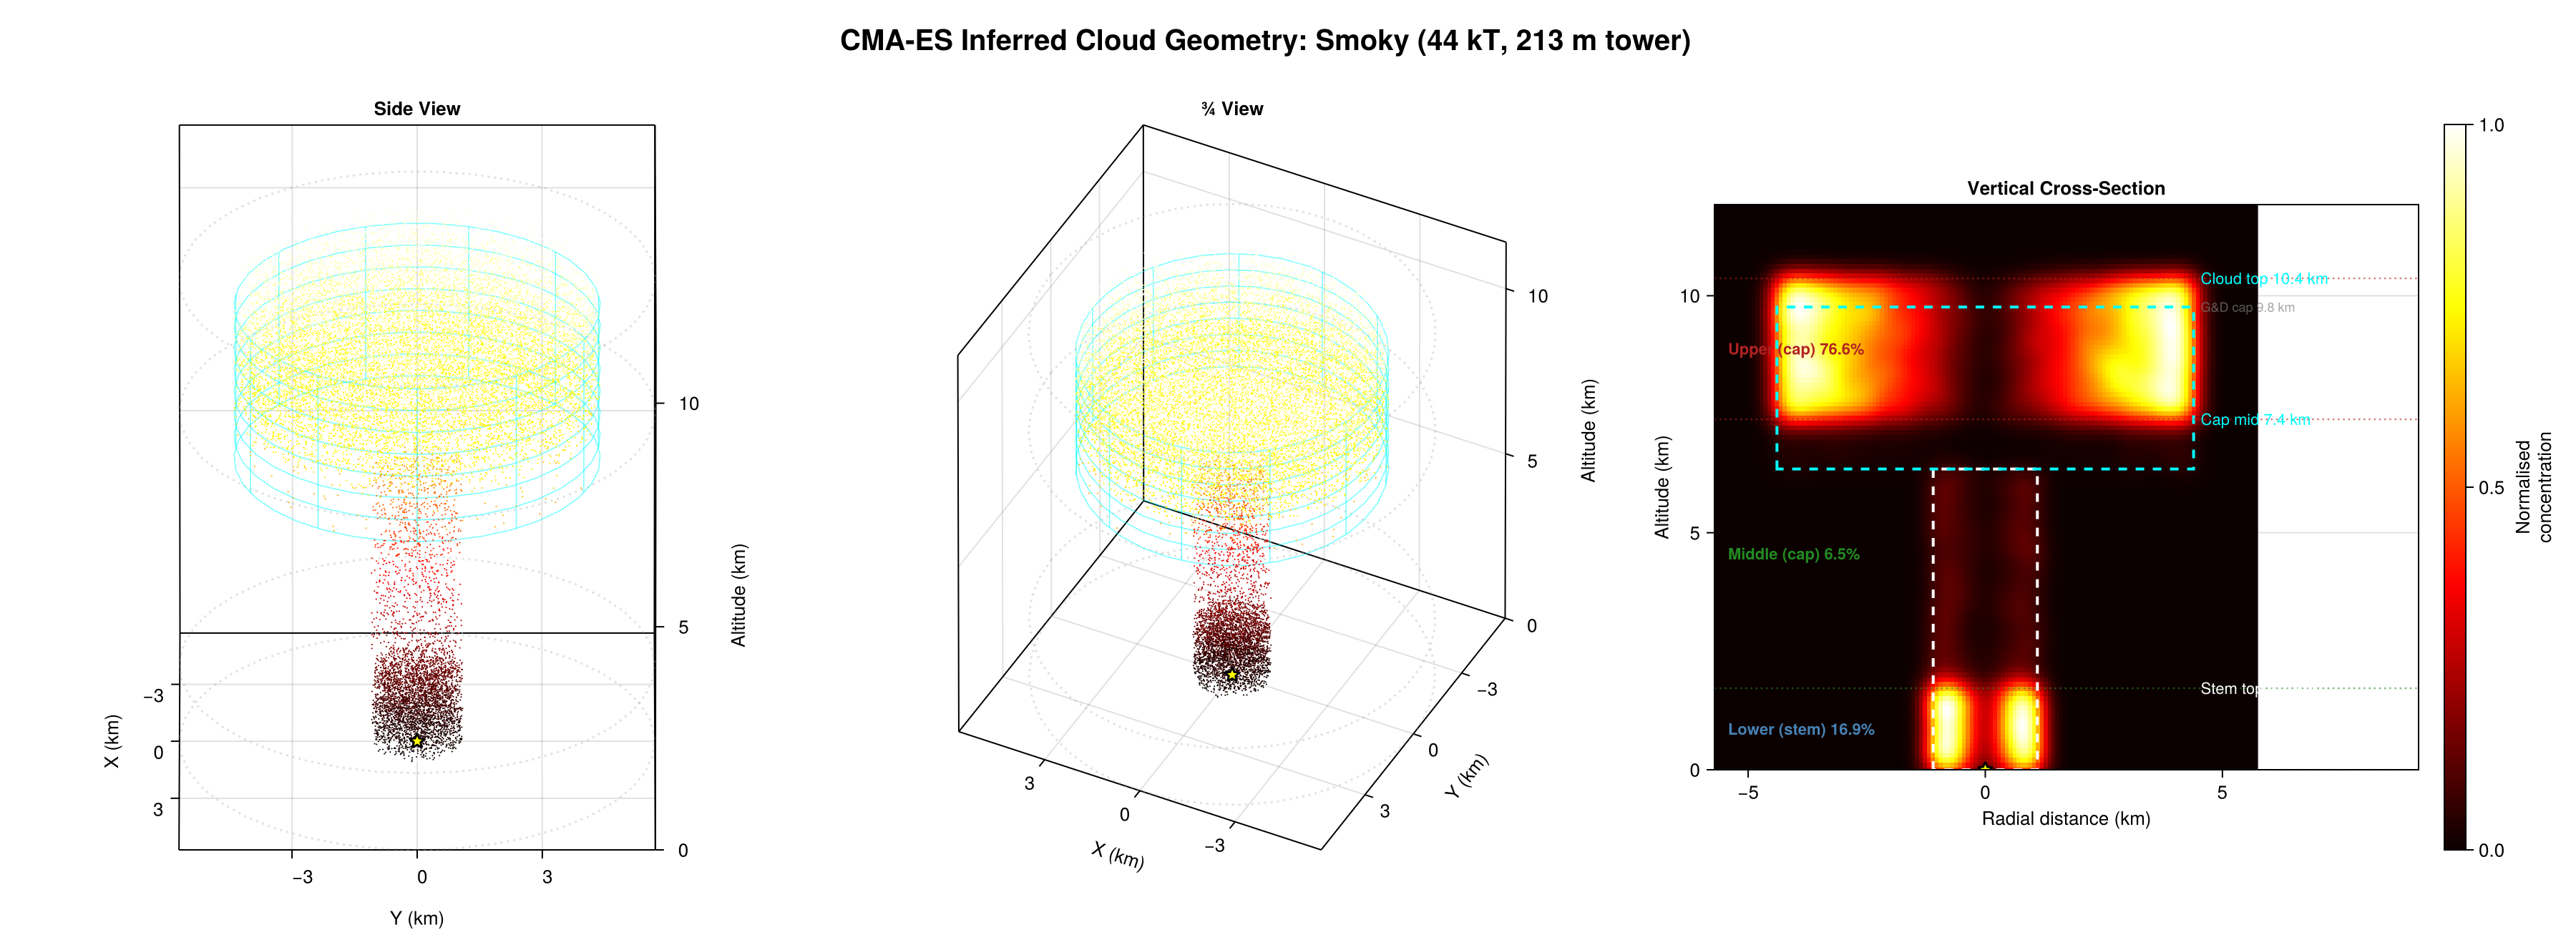
\includegraphics[width=\textwidth]{smoky_mushroom_cloud.png}
\caption{Smoky 44\,kT CMA-ES-inferred release geometry. Three-layer
particle distribution (lower 16.9\%, middle 6.5\%, upper 76.6\%) with
coloured wireframes showing the optimised cylinder boundaries. Thin grey
outlines show the Glasstone \& Dolan empirical cloud for reference.}
\label{fig:smoky_cloud}
\end{figure}

Table~\ref{tab:smoky_fms} presents the per-threshold FMS scores for Smoky.
The current best parameter set achieves a geometric-mean FMS of 44.7\%, with
the modelled plume correctly reproducing the eastward fallout lobe driven by
mid-tropospheric westerlies documented in DNA~6004F. Consortium submissions
for Smoky are pending; columns are reserved for comparison once results
become available. Calibration is ongoing and we expect further improvement
as the parameter space is explored.

\begin{table}[htbp]
\centering
\caption{FMS scores for Smoky 44\,kT at H+12. Consortium results are
pending.}
\label{tab:smoky_fms}
\begin{tabular}{lrrrrrr}
\toprule
Dose Rate (mR/h) & Our Model & UKMO & BfS & KIT & DSA/MET & DEMA \\
\midrule
1 & 47.4\% & & & & & \\
10 & 44.8\% & & & & & \\
50 & 54.4\% & & & & & \\
100 & 52.5\% & & & & & \\
500 & 40.2\% & & & & & \\
1000 & 32.7\% & & & & & \\
\midrule
Geo.\ mean & \textbf{44.7\%} & & & & & \\
\bottomrule
\end{tabular}
\end{table}

Figure~\ref{fig:smoky} compares observed and modelled fields for both dose
rate and time of arrival. The dose rate contours (top row) show the ESE
plume axis is well captured, whilst the TOA contours (bottom row) demonstrate
that the plume advances at the correct speed, with model H+1 through H+12
contours progressing downwind in agreement with the DASA-1251 \cite{dasa1251} survey arcs.

\begin{figure}[htbp]
\centering
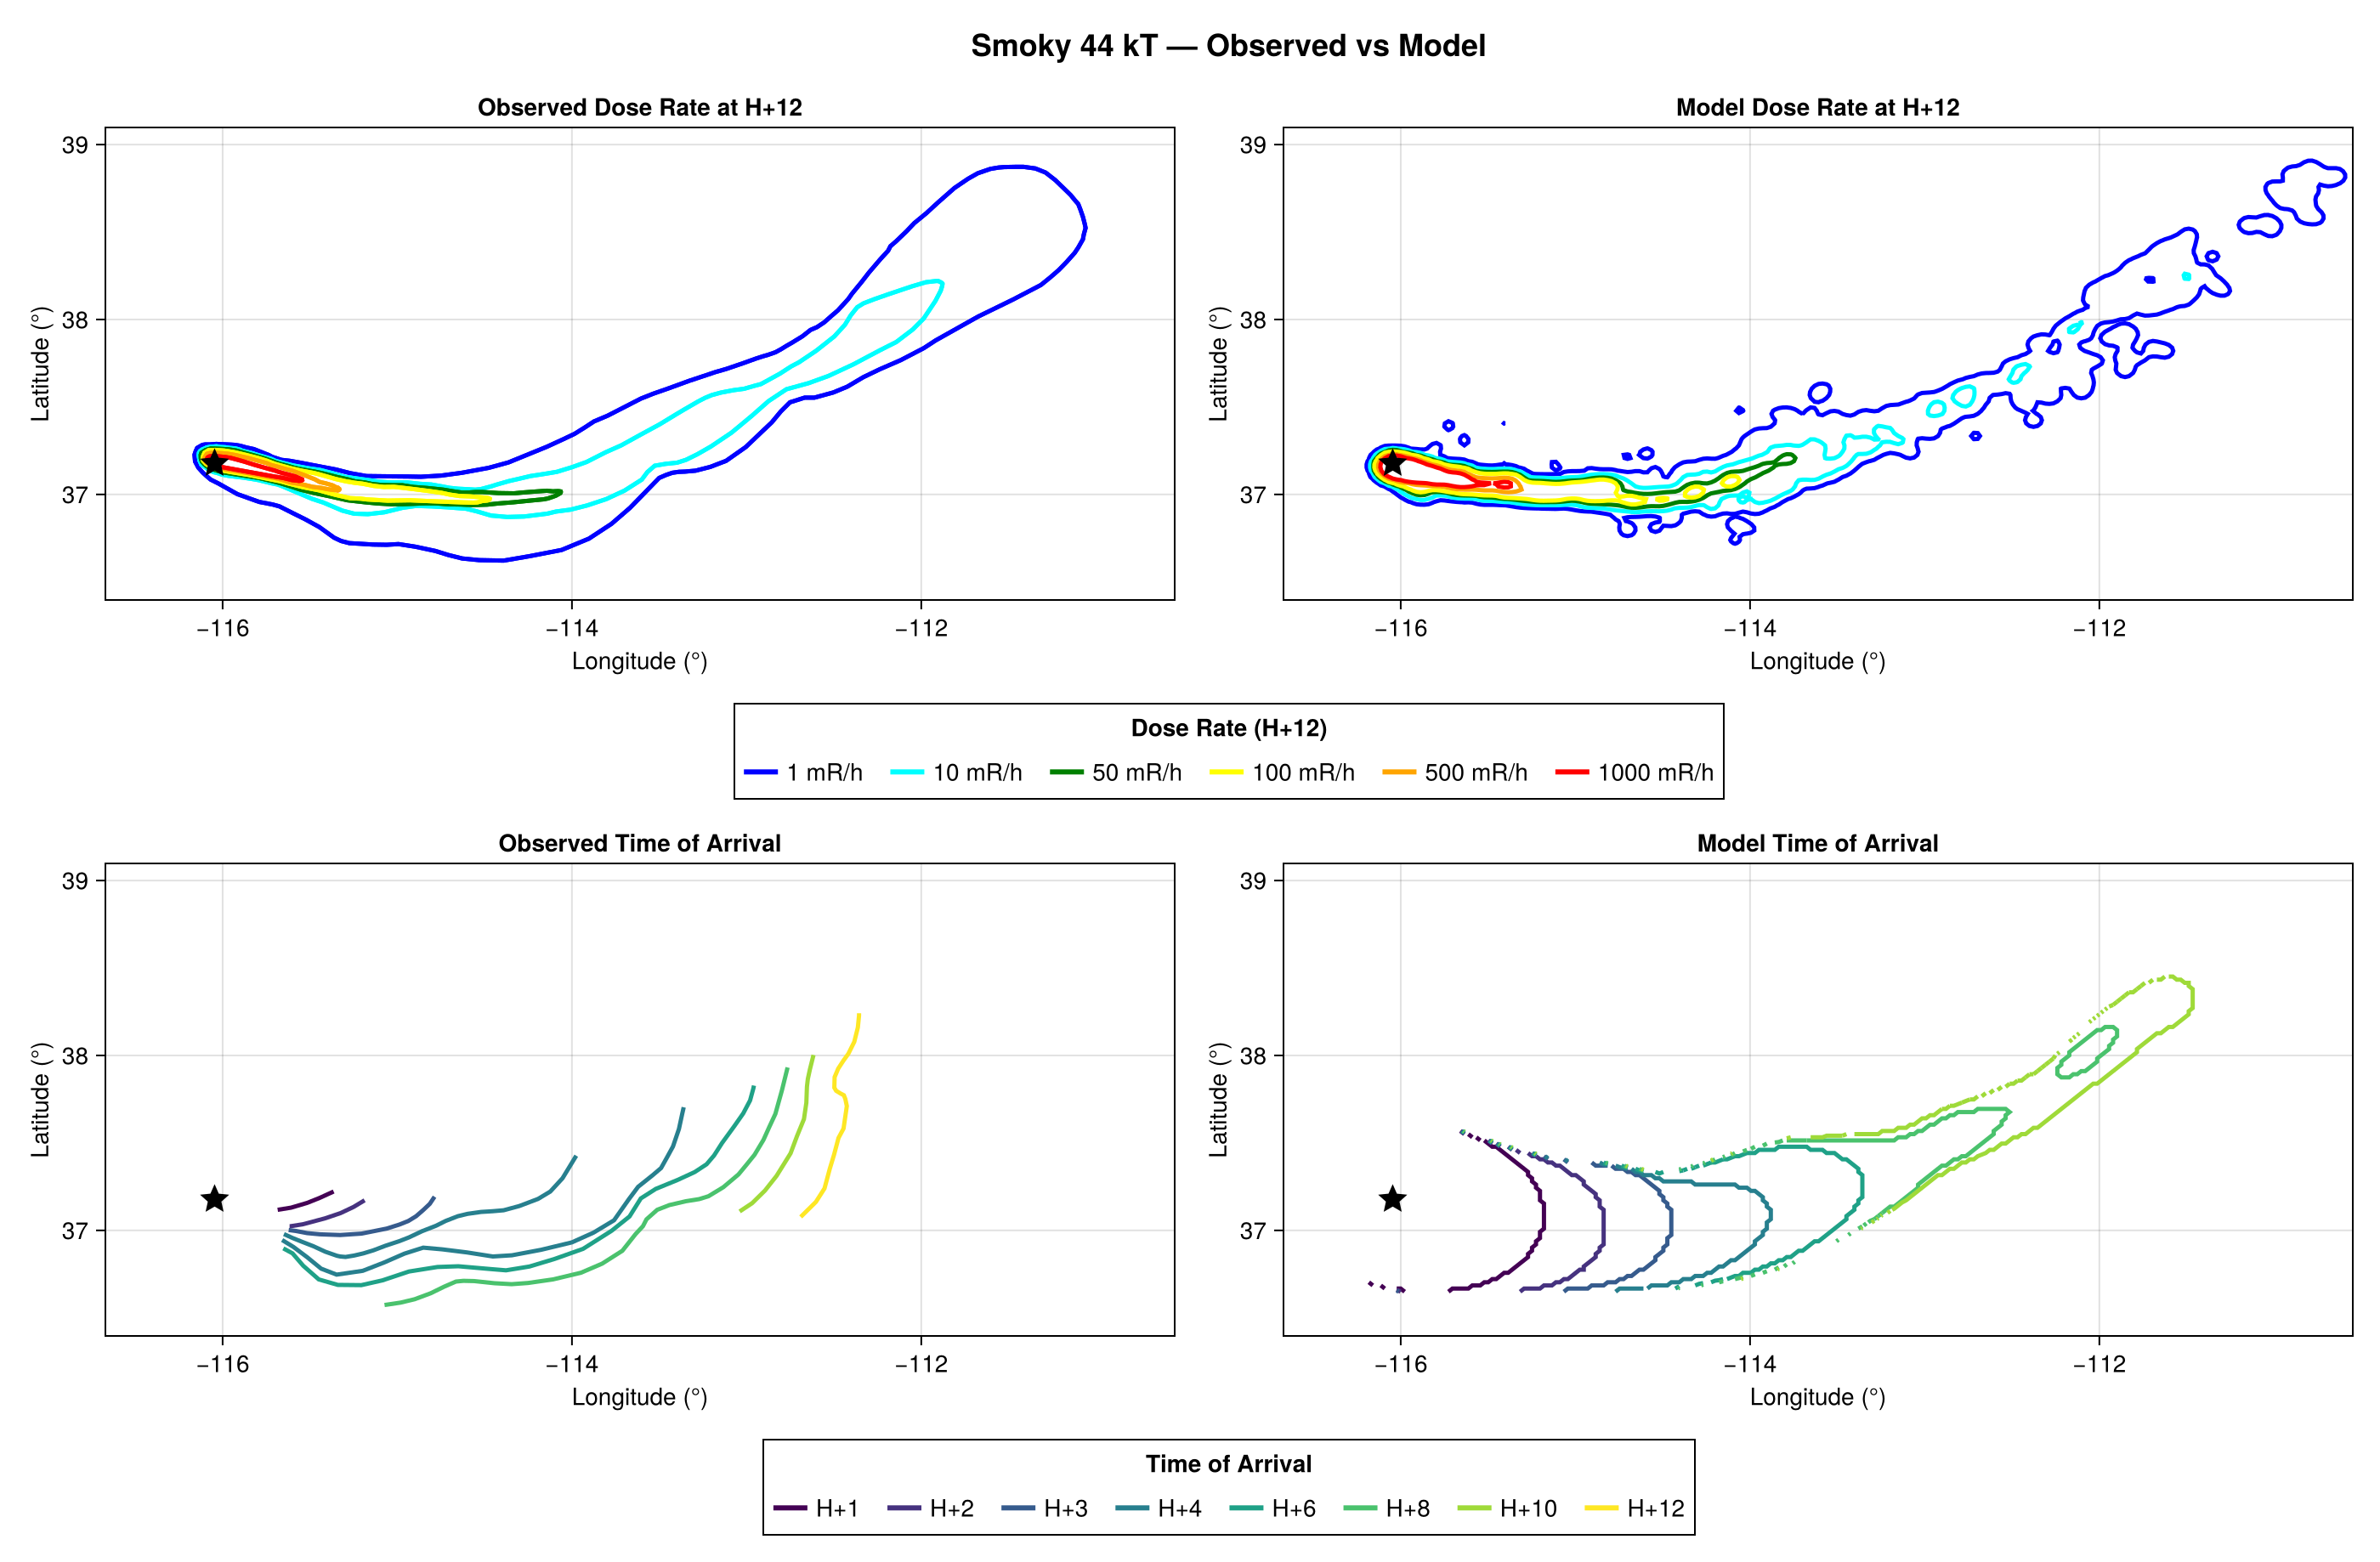
\includegraphics[width=\textwidth]{smoky_bomb_release.png}
\caption{Smoky 44\,kT: observed (left) vs model (right). Top row: dose
rate contours at H+12 for six thresholds (1, 10, 50, 100, 500,
1000\,mR/h). Bottom row: time-of-arrival contours showing plume
progression from H+1 through H+12.}
\label{fig:smoky}
\end{figure}

%% ====================================================================
%% Parameter comparison section commented out per Robert's feedback
%% ====================================================================
% \clearpage
% \section{Parameter Comparison: Nancy vs Smoky}
% \label{sec:comparison}
%
% Both tests were independently optimised via BIPOP-CMA-ES against digitised
% fallout observations, reaching combined scores of approximately 77\%.
% Comparing the best-fit parameters (Table~\ref{tab:param_compare} and
% Figure~\ref{fig:param_compare}) reveals which physics are robust across
% tests versus test-specific.
%
% \begin{table}[htbp]
% \centering
% \caption{Best-fit parameter comparison: Nancy 24\,kT vs Smoky 44\,kT
% (OU turbulence). Parameters grouped by category.}
% \label{tab:param_compare}
% \small
% \begin{tabular}{llrrr}
% \toprule
% Parameter & Physical meaning & Nancy & Smoky & Units \\
% \midrule
% \multicolumn{5}{l}{\textit{Particle size}} \\
% $d_\text{fine}$           & Fine mode median diameter     & 127.6 & 83.4  & \si{\micro\metre} \\
% $\sigma_{g,\text{fine}}$  & Fine mode geometric std dev   & 2.67  & 2.81  & -- \\
% $d_\text{coarse}$         & Coarse mode median diameter   & 141.9 & 100.7 & \si{\micro\metre} \\
% $\sigma_{g,\text{coarse}}$& Coarse mode geometric std dev & 2.52  & 2.80  & -- \\
% $f_\text{fine}$           & Fine mode mass fraction       & 86.5\% & 45.6\% & -- \\
% \midrule
% \multicolumn{5}{l}{\textit{Layer fractions}} \\
% $f_\text{lower}$          & Lower layer mass fraction     & 5.6\% & 16.9\% & -- \\
% $f_\text{middle}$         & Middle layer mass fraction    & 35.1\% & 6.5\% & -- \\
% \midrule
% \multicolumn{5}{l}{\textit{Turbulence}} \\
% $\sigma_w$                & Vertical diffusivity scale    & 4.03  & 4.81  & $\times$ \\
% $\sigma_h$                & Horizontal diffusivity scale  & 2.22  & 2.97  & $\times$ \\
% $K_h$                     & Horiz.\ diffusion in BL       & 0.21  & 1.23  & $\times$ \\
% $\tau_L$                  & Lagrangian timescale          & 4.46  & 2.05  & $\times$ \\
% \midrule
% \multicolumn{5}{l}{\textit{Physics}} \\
% $v_d$                     & Dry deposition velocity       & 4.40  & 3.02  & $\times$ \\
% $v_g$                     & Gravitational settling        & 0.55  & 4.44  & $\times$ \\
% $\omega$                  & ERA5 vertical velocity        & 2.56  & 2.41  & $\times$ \\
% $h_\text{mix}$            & BL mixing height              & 4.11  & 4.40  & $\times$ \\
% $\tau_\text{mix}$         & Mixing timescale              & 1.29  & 0.75  & $\times$ \\
% \midrule
% \multicolumn{5}{l}{\textit{Deposition}} \\
% $h_\text{sfc}$            & Surface height scale          & 1.55  & 9.52  & $\times$ \\
% $z_0$                     & Surface roughness             & 1.17  & 3.59  & $\times$ \\
% \midrule
% \multicolumn{5}{l}{\textit{Calibration}} \\
% $A$                       & Total release activity        & 48.4  & 302.7 & $\times 10^{15}$\,Bq \\
% $\sigma_s$                & Gaussian smoothing width      & 2.17  & 1.46  & cells \\
% \bottomrule
% \end{tabular}
% \end{table}
%
% \begin{figure}[htbp]
% \centering
% 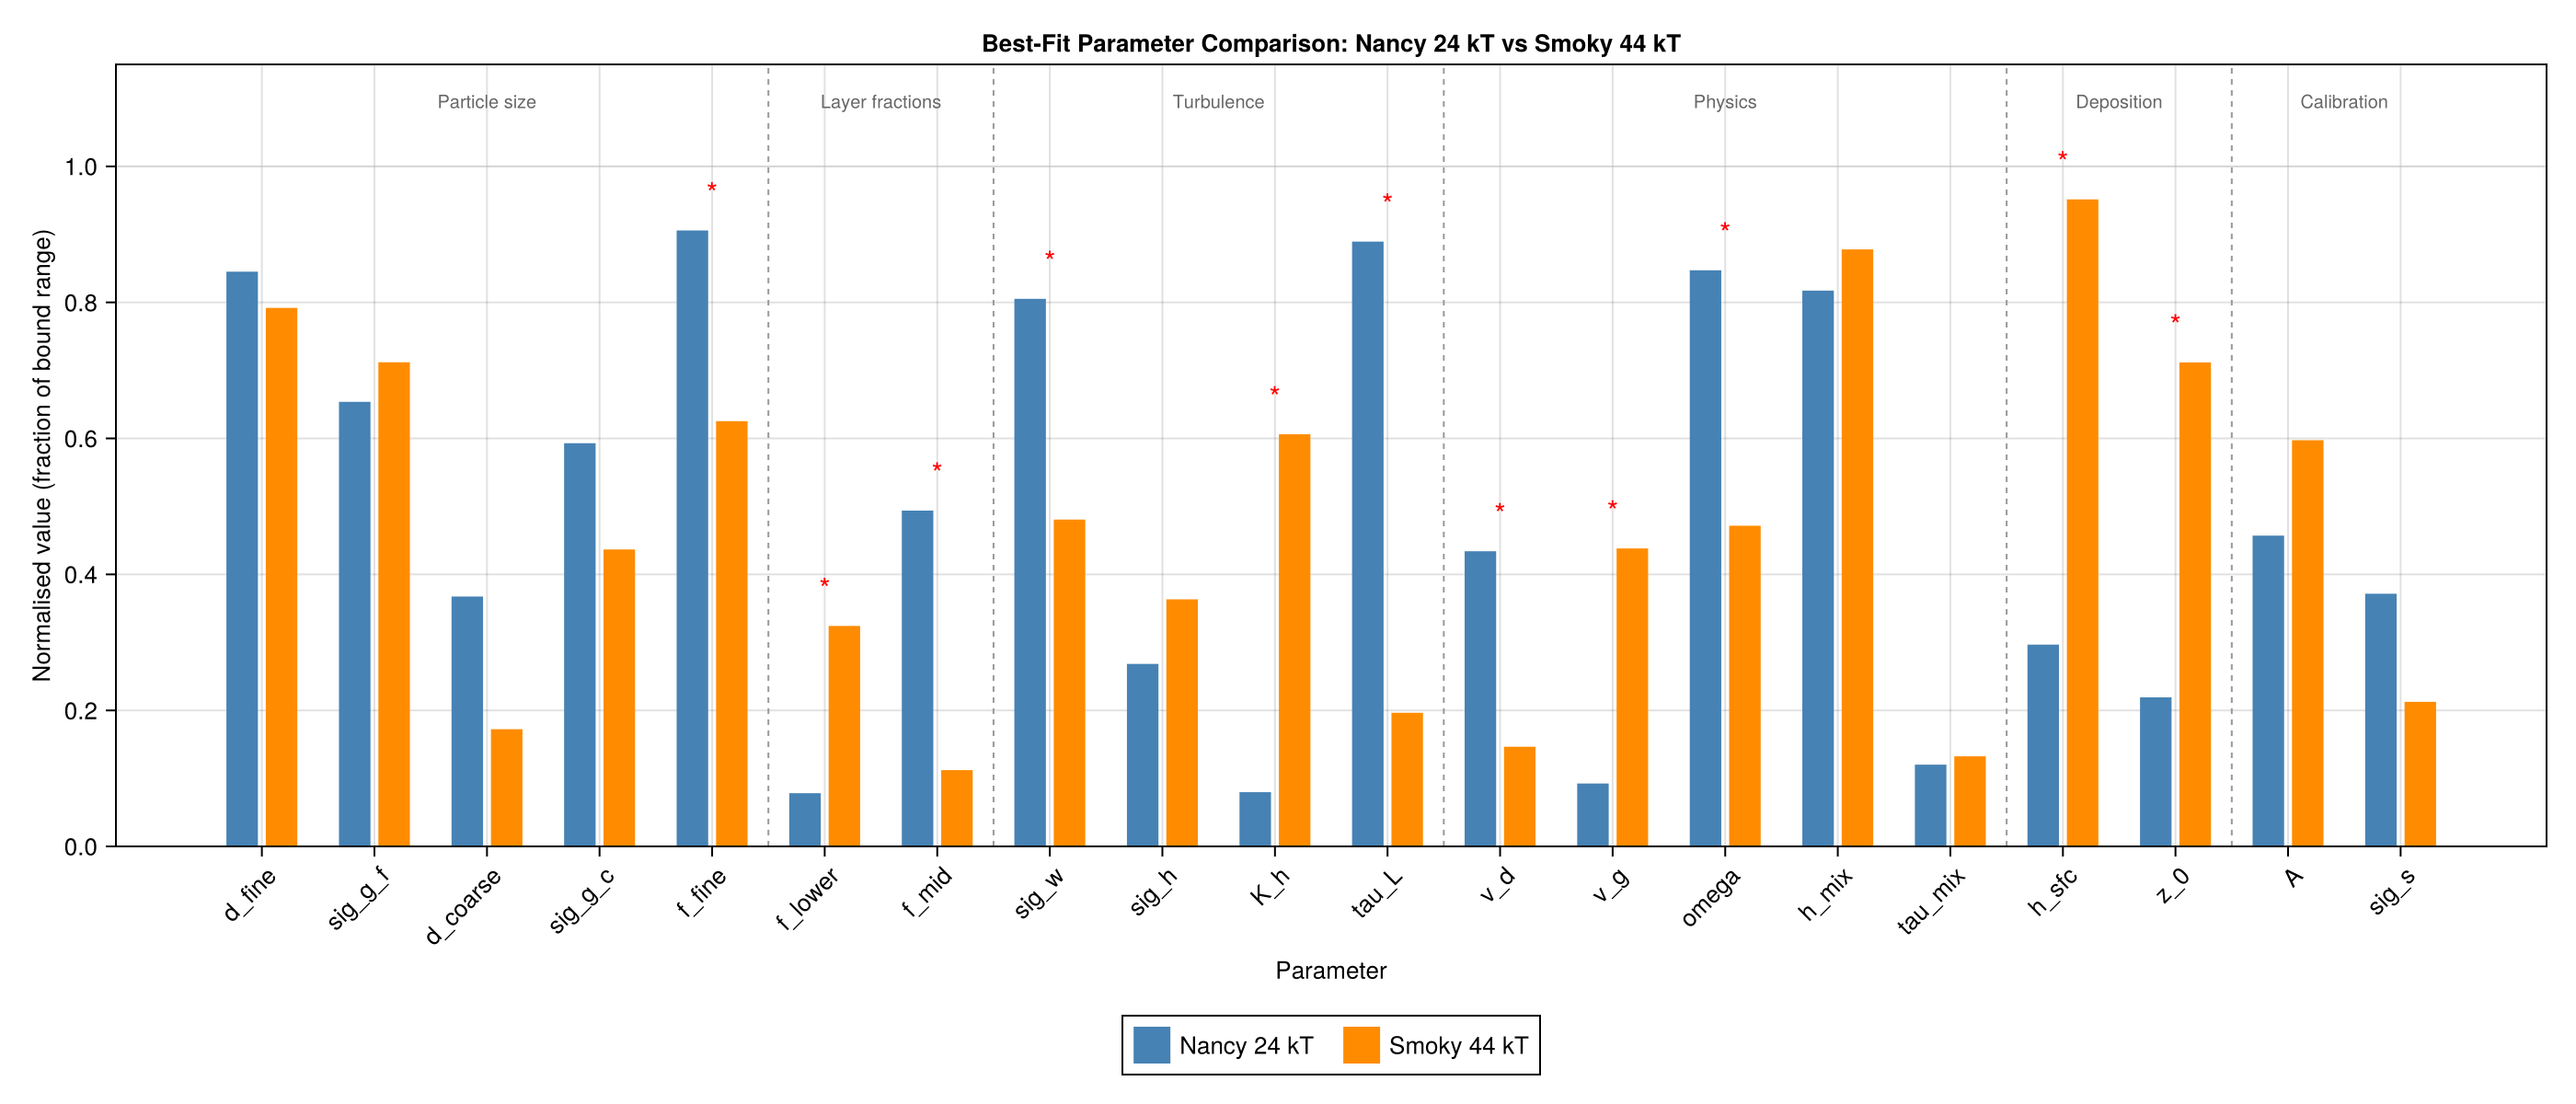
\includegraphics[width=\textwidth]{param_comparison.png}
% \caption{Normalised parameter comparison: Nancy (blue) vs Smoky (orange).
% Each bar shows the parameter's position within its optimisation bound range
% (0\% = lower bound, 100\% = upper bound). Red asterisks mark parameters
% where the two tests diverge by more than 20\% of the bound range.}
% \label{fig:param_compare}
% \end{figure}
%
% \subsection{Consistent Parameters}
%
% Several parameters converge to similar values across both tests, suggesting
% that they capture robust atmospheric physics rather than test-specific
% tuning. The ERA5 vertical velocity scaling factor $\omega$ settles at
% $2.4$--$2.6\times$ in both cases, implying a systematic low bias in the
% reanalysis resolved vertical motion for 1950s NTS conditions. This is
% consistent with the coarse ERA5 grid ($\sim$30\,km) being unable to resolve
% the mesoscale convergence zones and mountain passes that channel debris
% transport across the Nevada landscape.
%
% The boundary-layer mixing height scale ($h_\text{mix} \approx
% 4.1$--$4.4\times$) is similarly consistent, indicating that the convective
% boundary layer over the Nevada desert grows deeper than the reanalysis
% represents. Intense surface heating in the arid terrain likely amplifies
% boundary-layer growth beyond what ERA5 resolves at its native resolution.
%
% The geometric standard deviations of both the fine and coarse particle
% modes ($\sigma_g \approx 2.5$--$2.8$) agree well between the two tests.
% This suggests that the lognormal spread of the particle size distribution
% is a generic feature of nuclear debris formation rather than something
% dependent on individual weapon design. Horizontal diffusivity
% ($\sigma_h \approx 2.2$--$3.0\times$) also requires moderate enhancement
% in both cases to reproduce the observed plume widths, pointing to
% sub-grid-scale turbulent mixing that the ERA5 wind fields alone cannot
% capture.
%
% \subsection{Divergent Parameters}
%
% Other parameters show large differences between the two tests, reflecting
% genuinely different physical conditions. The most striking divergence is in
% gravitational settling: the Nancy optimisation suppresses settling
% ($v_g = 0.55\times$), keeping fine particles aloft over long distances,
% whereas Smoky enhances it strongly ($v_g = 4.4\times$), depositing coarse
% material quickly. This is consistent with the fine-mode mass fraction,
% which the optimiser places at 86.5\% for Nancy but only 45.6\% for Smoky.
% Nancy's fallout pattern is therefore dominated by fine particles that
% travel far downwind, whilst Smoky's substantial coarse fraction produces
% heavier near-field deposition. The difference may reflect the two weapon
% designs: Nancy was a relatively small 24\,kT device, possibly generating
% finer debris, whilst Smoky's larger 44\,kT yield and tower-shot geometry
% lofted considerably more soil material into the coarse fraction.
%
% The Lagrangian timescale $\tau_L$ also diverges markedly, with Nancy at
% $4.5\times$ and Smoky at $2.0\times$. A longer timescale preserves plume
% coherence over greater distances, which is consistent with the narrow,
% elongated fallout pattern observed for Nancy. Smoky's shorter timescale
% produces more vigorous local mixing that broadens the plume, matching the
% wider deposition footprint recorded in the DASA-1251 surveys.
%
% The surface height scale ($h_\text{sfc}$: Nancy 1.6 vs Smoky 9.5) shows a
% large difference that likely compensates for the different effective terrain
% roughness experienced by the two plumes as they traverse different sectors
% of the NTS landscape. It may also absorb systematic meteorological
% differences between the March 1953 and August 1957 events. The lower-layer
% mass fraction ($f_\text{lower}$: Nancy 5.6\% vs Smoky 16.9\%) is
% consistent with Smoky's larger yield producing more low-altitude stem
% debris, as documented in the DASA-1251 observation that Smoky's stem was
% more prominent relative to its cap.
%
% \subsection{Physical Implications}
%
% The consistent $\sim$2.5$\times$ vertical velocity scaling across both
% tests points to a systematic ERA5 bias for 1950s NTS conditions. The
% reanalysis grid is too coarse to resolve the narrow mountain valleys and
% passes through which debris was channelled, and consequently underestimates
% the true mesoscale vertical motion. This finding has practical implications
% for any future dispersion modelling over complex terrain using ERA5: a
% correction factor of approximately 2.5 for resolved omega appears
% necessary to reproduce observed fallout patterns.
%
% The particle size divergence between the tests (Nancy dominated by fine
% particles with suppressed settling, Smoky by a mixed distribution with
% enhanced settling) may reflect genuine differences in weapon design,
% including fission fraction, casing material, and burst geometry. The total
% activity ratio ($302.7 / 48.4 \approx 6.3\times$) is considerably larger
% than the simple yield ratio ($44 / 24 = 1.8\times$), suggesting either
% that Smoky had a higher fission efficiency or that its tower-shot geometry
% entrained substantially more activated soil into the debris cloud. Further
% work comparing against additional NTS tests would help disentangle
% yield-dependent from geometry-dependent effects.

%% ====================================================================
\begin{thebibliography}{9}

\bibitem{dasa1251}
H.~A.~Hawthorne,
\textit{Compilation of Local Fallout Data from Test Detonations
1945--1962, Extracted from DASA~1251},
Vols.~I and II, General Electric Co.--TEMPO, Defense Nuclear Agency,
1979.

\bibitem{uhlenbeck1930}
G.~E.~Uhlenbeck and L.~S.~Ornstein,
``On the Theory of the Brownian Motion,''
\textit{Physical Review}, vol.~36, no.~5, pp.~823--841, 1930.

\bibitem{cunningham1910}
E.~Cunningham,
``On the velocity of steady fall of spherical particles through fluid
medium,''
\textit{Proceedings of the Royal Society A}, vol.~83, no.~563,
pp.~357--365, 1910.

\bibitem{sutherland1893}
W.~Sutherland,
``The viscosity of gases and molecular force,''
\textit{The London, Edinburgh, and Dublin Philosophical Magazine and
Journal of Science}, vol.~36, no.~223, pp.~507--531, 1893.

\bibitem{zhang2001}
L.~Zhang, S.~Gong, J.~Padro, and L.~Barrie,
``A size-segregated particle dry deposition scheme for an atmospheric
aerosol module,''
\textit{Atmospheric Environment}, vol.~35, no.~3, pp.~549--560, 2001.

\end{thebibliography}

\end{document}
